% EMSE submission, Springer svjour3 class (smallcondensed).
% svjour3.cls v3.2 + svglov3.clo obtained from Springer's svjour3
% distribution. Bibliography: Springer's spbasic.bst is not freely
% redistributable; abbrvnat (author-year, visually close) is used here --
% swap \bibliographystyle{abbrvnat} for {spbasic} on Overleaf/at submission.
\documentclass[smallcondensed]{svjour3}
\journalname{Empirical Software Engineering}

\smartqed

\usepackage[T1]{fontenc}
\usepackage{mathptmx}
\usepackage{graphicx}
\usepackage{booktabs}
\usepackage{multirow}
\usepackage{amsmath}
\usepackage{amssymb}
\usepackage{xspace}
\usepackage[round,authoryear]{natbib}
\usepackage{enumitem}
\setlist{topsep=2pt,itemsep=1pt,leftmargin=1.4em}
\usepackage{tcolorbox}
\usepackage[hidelinks]{hyperref}

\newtcolorbox{findingbox}{colback=black!4!white, colframe=black!60!white,
  boxrule=0.5pt, arc=1.5pt, left=6pt, right=6pt, top=4pt, bottom=4pt,
  before skip=8pt, after skip=8pt}

\newcommand{\srs}{SRS\xspace}
\newcommand{\pilotcost}{\textsf{pilotCost}\xspace}
\newcommand{\diShe}{\textsf{diversity}\xspace}
\newcommand{\randomS}{\textsf{random}\xspace}
\newcommand{\pairwise}{\textsf{pairwise}\xspace}
\newcommand{\balanced}{\textsf{balanced}\xspace}
\newcommand{\finding}[1]{\begin{findingbox}\small\textbf{#1}\end{findingbox}}
\newcommand{\rqone}{RQ\textsubscript{1}\xspace}
\newcommand{\rqtwo}{RQ\textsubscript{2}\xspace}

\begin{document}

\title{Replicating Posterior Guarantees of Configuration Sampling
Strategies under Measured Acquisition Cost}
\titlerunning{Posterior Guarantees under Measured Acquisition Cost}

\author{Mathieu Acher \and Juliana Alves Pereira \and Th\'eo Matricon}
\authorrunning{M. Acher et al.}

\institute{M. Acher \and T. Matricon \at
  Univ Rennes, Inria, CNRS, IRISA, Rennes, France\\
  \email{mathieu.acher@irisa.fr}, \email{theo.matricon@irisa.fr}%% TODO: verify T. Matricon affiliation/email
  \and
  J. Alves Pereira \at
  Pontifical Catholic University of Rio de Janeiro (PUC-Rio), Rio de
  Janeiro, Brazil\\
  \email{juliana@inf.puc-rio.br}%% TODO: verify
}

\date{Received: date / Accepted: date}

\maketitle

\begin{abstract}
Practitioners of configurable software systems rely on budgeted sampling
strategies to estimate worst-case (or best-case) performance bounds. A
recent FSE~2026 study introduced \emph{posterior risk} and
\emph{posterior confidence} as learner-free, scenario-theoretic
guarantees for such sampled bounds, and found that Statistical Recursive
Search (\srs) consistently yields tighter guarantees than alternative
strategies at the same sample size. We replicate this study on its
original artifact and extend it to five further dataset families---851
decision scopes across six corpora---and then re-index every decision by
\emph{measured acquisition cost} instead of sample size. The guarantee
framework replicates everywhere: posterior-risk distributions
discriminate strategies in about 95\% of scopes, robust to
false-discovery-rate correction. The strategy recommendation, however, is
population-relative: \srs{} dominates on the original systems and on an
x264 corpus, but is never the best cost-normalized choice on Linux kernel
or hyperparameter-optimization pools. Under measured cost, the
guarantee/cost Pareto frontier differs from the sample-size frontier in
97.5\% of scopes. Two equal-spend experiments explain these boundaries:
cost-aware sampling helps exactly when acquisition cost is decoupled from
the bounded target (its verdict flips from $6.6\times$ worse to better
than random as the coupling weakens), and \srs's advantage requires
budget to amortize. Posterior guarantees are thus a sound and portable
evaluation framework, but strategy recommendations---including which
strategy is ``cost-effective''---depend on the outcome, the budget scale,
and the cost--target coupling, none of which sample size can express.
\keywords{Configurable systems \and Sampling strategies \and Performance
bounds \and Scenario theory \and Replication \and Measurement cost}
\end{abstract}

\section{Introduction}
\label{sec:intro}

Modern software systems expose hundreds to thousands of configuration
options, and the chosen configuration can change performance---execution
time, energy consumption, binary size---by orders of magnitude
\citep{xu2015hey,apel2013feature,pereira2021learning}. For many
engineering tasks the question is not what performance a \emph{typical}
configuration exhibits, but how bad (or how good) performance can get:
worst-case execution time for safety arguments, best-case throughput for
capacity planning, largest kernel size for resource-constrained
deployment. Exhaustive measurement is infeasible even for moderately
sized spaces, so practitioners sample: they measure a budgeted subset of
configurations and use the observed extremum as a proxy for the true
bound.

How trustworthy is such a sampled bound? A recent FSE~2026 study by
\citet{weis2026risk} gives this question a rigorous footing. Building on
scenario theory \citep{calafiore2006scenario,campi2008exact}, it defines
the \emph{posterior risk} of a sampled bound---the empirical probability
that an unseen configuration violates it---and the \emph{posterior
confidence} that the risk stays below a tolerance. These measures are
computed directly from measurements, with no learned model anywhere in
the loop, and they turn strategy comparison into a quantitative exercise:
at the same sample size, which strategy delivers lower risk and higher
confidence? Across five strategies and seven real-world configurable
systems, \citet{weis2026risk} find that Statistical Recursive Search
(\srs) \citep{oh2017srs} ``yields consistently tighter best-case
guarantees---higher posterior confidence and lower posterior risk---than
the alternatives at the same budget,'' while plain solver-based sampling
proves least reliable.

This paper starts from a construct-validity observation about the phrase
\emph{at the same budget}. Like virtually all sampling studies of
configurable systems
\citep{kaltenecker2019distance,pereira2020sampling,guo2018dataefficient},
the FSE study equates budget with \emph{sample size}: strategies are
compared after acquiring the same number of configurations. But
configurations are not interchangeable units of effort. Measuring a
slow, energy-hungry, or large configuration costs more---in wall-clock
time, in joules, in compute dollars---than measuring a cheap one, and
sampling strategies differ systematically in which configurations they
select; indeed, an entire line of strategy design exploits exactly this
asymmetry \citep{sarkar2015cost,nair2017bad}. Whether strategy
\emph{evaluations}, and the recommendations built on them, survive the
switch from counted samples to measured spend has not been examined for
guarantee-oriented sampling---and guarantees are arguably where the
question matters most, because a practitioner who buys a worst-case bound
is typically operating under an explicit measurement budget.

Posterior guarantees are also the sharpest possible place to test such a
cost argument. Studies whose outcome is prediction error entangle the
sampling strategy with a learner, and conclusions can shift with the
choice of regressor \citep{kaltenecker2020interplay}. Posterior risk has
no learner: sample, take the extremum, count violations. Any decision
change we observe when re-indexing by cost is attributable to the cost
construct alone (Figure~\ref{fig:bridge} illustrates the argument).

\begin{figure}[t]
  \centering
  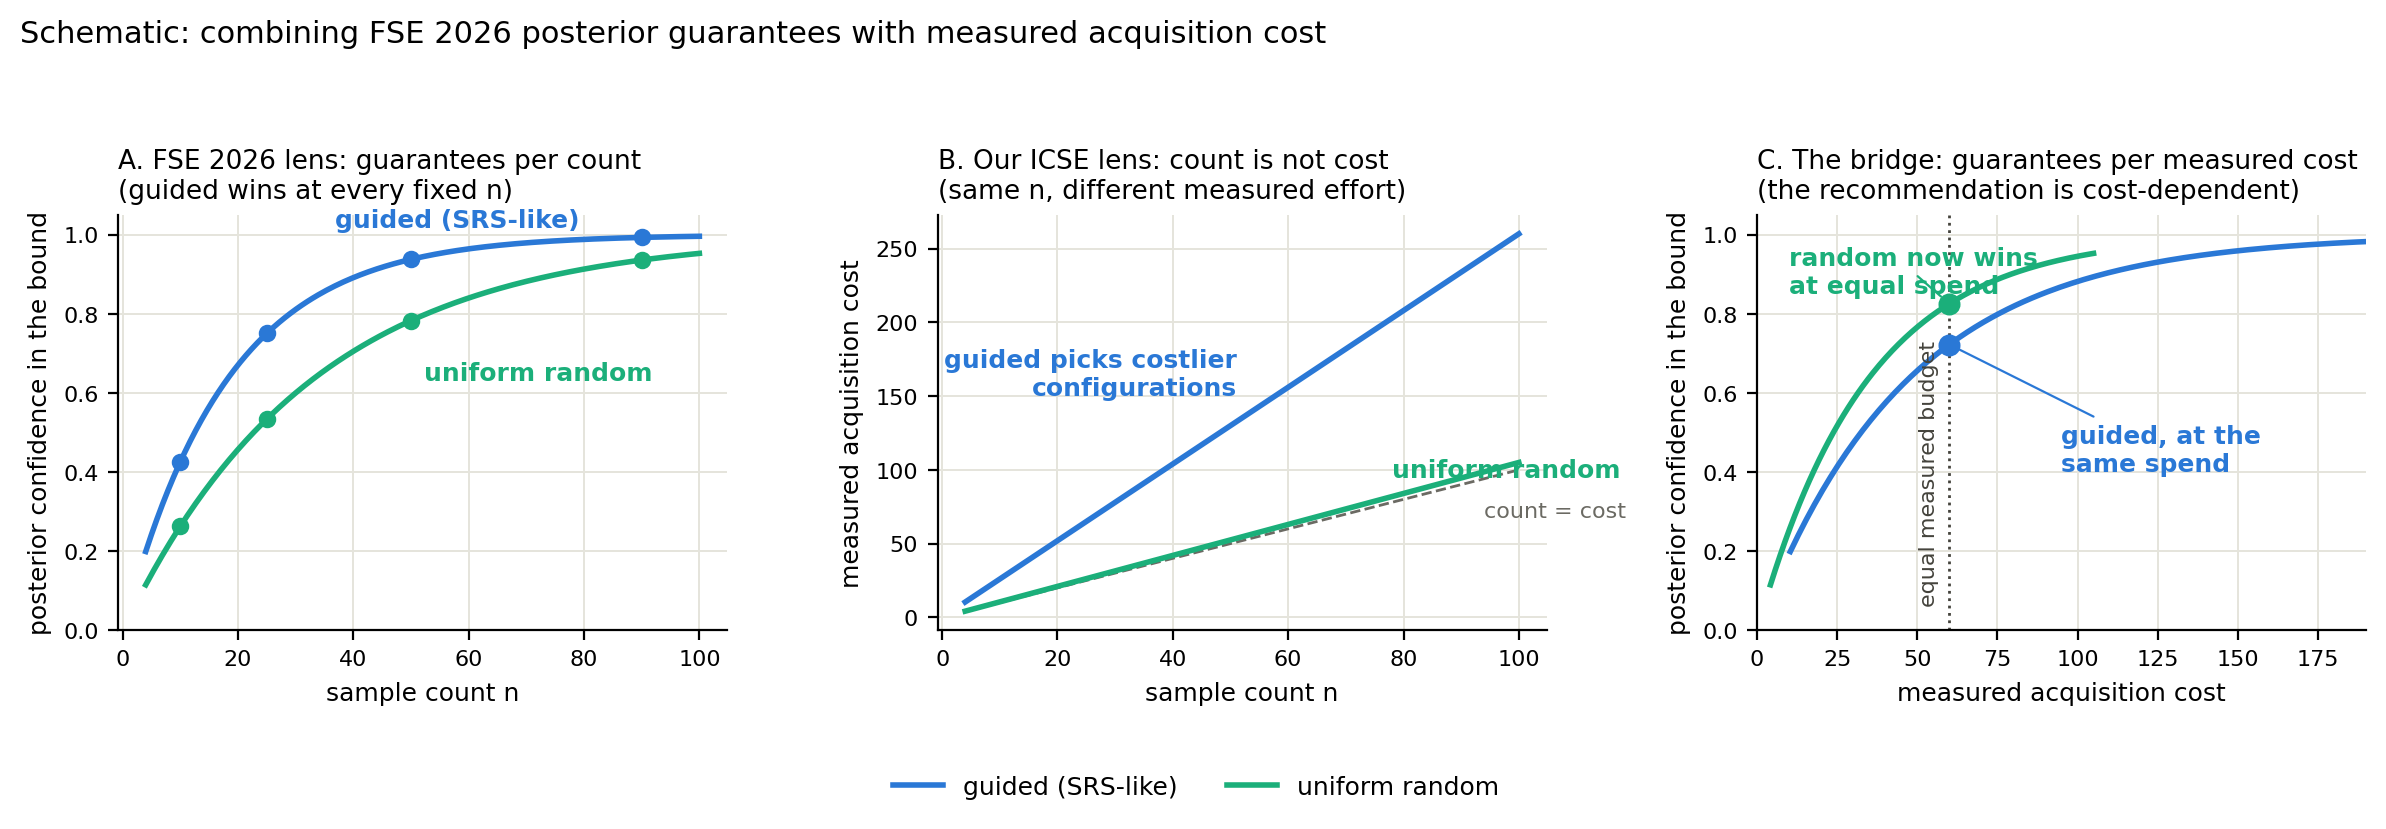
\includegraphics[width=\linewidth]{figures/fig_bridge_concept.png}
  \caption{Schematic of the studied question. (A)~At a fixed sample
  count, a guided strategy such as \srs{} achieves better guarantees than
  uniform random sampling---the FSE~2026 lens. (B)~The same sample count
  can correspond to very different measured acquisition costs.
  (C)~Re-indexing guarantees by measured cost changes the decision
  surface: at an equal measured budget, the recommendation can flip.}
  \label{fig:bridge}
\end{figure}

We therefore conduct a large-scale conceptual replication and extension
of \citet{weis2026risk}, organized around two research questions:

\begin{description}
\item[\rqone:] \emph{Do the FSE~2026 core claims replicate beyond the
  original artifact, at the paper's own fixed-sample-size lens?} We
  decompose this into four sub-questions mirroring the original claims:
  discriminative power of posterior risk, monotone improvement with
  budget, \srs{} superiority, and solver-based unreliability.
\item[\rqtwo:] \emph{Do the FSE~2026 metrics survive re-indexing by
  measured sampling cost instead of sample size?} We decompose this along
  a cost-validity lens: cost heterogeneity at fixed size, calibration of
  size as a cost proxy, impact on recommendations and Pareto frontiers,
  cost-normalized strategy choice, and an explicit equal-spend protocol
  in which strategies literally spend the same measured budget.
\end{description}

Our study spans six corpora: the original FSE artifact (direct data
reuse, seven systems), the x264 corpus of the ICPE'20 replication study
\citep{pereira2020sampling}, fourteen systems with measured energy and
runtime \citep{weber2023twins}, nine systems across all ninety-three
workloads of the ICSE'23 workload study \citep{muehlbauer2023workload},
seven Linux kernel releases \citep{martin2022transfer}, and thirty-five
hyperparameter-optimization pools \citep{zimmer2021autopytorch}---851
(context~$\times$~budget) decision scopes in total.

\paragraph{Findings.} The guarantee \emph{framework} replicates
everywhere: posterior-risk distributions discriminate strategies in
$\approx$95\% of scopes, robust to false-discovery-rate correction. The
strategy \emph{recommendation} replicates only within the original
population: \srs{} dominates on the original systems and on x264, but is
never the best cost-normalized choice on the Linux and
hyperparameter-optimization pools, and rarely so on the energy and
workload families. Under measured cost, the guarantee/cost Pareto
frontier differs from the sample-size frontier in 97.5\% of the 851
scopes---the single most robust effect in our data---while the single top
recommendation changes in 27\%. Two dedicated equal-spend experiments
explain the boundaries mechanistically: a cost-aware strategy designed to
stretch measurement budgets is counterproductive for bounds exactly when
acquisition cost correlates with the target (its equal-spend verdict
flips from $6.6\times$ worse than random to \emph{better} than random as
the coupling weakens), and \srs's advantage requires budget to amortize
(from 4\% of scopes at the smallest budgets to 77\% at the largest).

\paragraph{Contributions.}
\begin{itemize}
\item A conceptual replication of \citet{weis2026risk} at unprecedented
  scale: six corpora, 851 decision scopes, with exact artifact reuse for
  the original systems and an audited reimplementation of \srs{}
  (behaviorally indistinguishable from the artifact, Mann--Whitney
  $p=0.95$).
\item A systematic re-indexing of posterior guarantees by measured
  acquisition cost---a construct-validity question that, to our
  knowledge, had not been examined for guarantee outcomes---at zero
  additional measurement cost, since every corpus already ships the
  required cost data.
\item Two equal-spend experiments (250 scopes) that identify the
  governing mechanisms: cost--target coupling and budget amortization.
  Together they show that ``cost-effective'' is a property of the triple
  (strategy, outcome, cost--target coupling), not of a strategy alone.
\item A fully scripted, checksummed replication package: per-corpus
  result tables, hypothesis tests with false-discovery-rate control, and
  a command-level manifest.
\end{itemize}

The remainder of the paper follows the structure of our research
questions: background and replicated claims
(Section~\ref{sec:background}), study design (Section~\ref{sec:design}),
replication results (Section~\ref{sec:rq1}), cost re-indexing results
(Section~\ref{sec:rq2}), discussion (Section~\ref{sec:discussion}),
threats (Section~\ref{sec:threats}), related work
(Section~\ref{sec:related}), and conclusions
(Section~\ref{sec:conclusion}).

\section{Background and Replicated Claims}
\label{sec:background}

\subsection{Sampling configuration spaces}

A configurable system with $k$ options spans a configuration space whose
valid members $\mathcal{V}$ are constrained by a variability model
\citep{apel2013feature}. A \emph{sampling strategy} selects a subset
$S \subseteq \mathcal{V}$, $|S| = n$, whose measurements serve a
downstream purpose: training a performance model
\citep{guo2013variability,siegmund2015performance,ha2019deepperf},
finding a near-optimal configuration \citep{oh2017srs,nair2020flash}, or,
in our setting, bounding worst-case (or best-case) performance. Strategy
families include uniform random sampling (in practice often
solver-mediated \citep{plazar2019uniform,heradio2022uniform}), coverage
oriented $t$-wise sampling \citep{medeiros2016comparison,baranov2024baital,hess2024unwise},
distance- and diversity-based sampling \citep{kaltenecker2019distance},
and adaptive strategies that use intermediate measurements to steer
selection \citep{sarkar2015cost,nair2017bad}.

\emph{Statistical Recursive Search} (\srs) \citep{oh2017srs}, the
strategy recommended by \citet{weis2026risk}, is adaptive: it repeatedly
draws a small random batch (25 configurations), identifies option
decisions shared by the two best configurations of the batch, keeps the
decisions whose enabled/disabled performance difference is significant
under Welch's $t$-test ($p<0.05$), restricts the space accordingly, and
recurses; if recursion stops before the budget is exhausted, the
remainder is filled with random configurations.

\subsection{Posterior risk and posterior confidence}
\label{sec:posterior}

Let $y(c)$ be the measured target of configuration $c \in \mathcal{V}$
and let $S$ be a sample. For a worst-case (maximum) bound, the sampled
bound is $\hat{b} = \max_{c \in S} y(c)$, and the \emph{posterior risk}
is the fraction of the reference universe that violates it:
\begin{equation}
  R(S) \;=\; \frac{\big|\{\,c \in \mathcal{V} : y(c) > \hat{b}\,\}\big|}{|\mathcal{V}|}.
  \label{eq:risk}
\end{equation}
Repeating the sampling $r$ times yields an empirical distribution of
risks; the \emph{posterior confidence} at tolerance $\varepsilon$ is the
fraction of repetitions with $R \le \varepsilon$, i.e., the empirical CDF
of risk. Integrating this CDF over $\varepsilon \in [0,1]$ gives the
\emph{integrated posterior confidence} $A_{\mathrm{post}} = 1 -
\overline{R}$, a scalar summary (higher is better). Scenario theory
provides a strategy-agnostic \emph{prior} baseline: for uniform random
samples of size $N$, confidence at tolerance $\varepsilon$ is
$1-(1-\varepsilon)^{N+1}$ (we follow the artifact's exponent convention
and report a sensitivity with exponent $N$). The \emph{integrated
confidence discrepancy} $\omega = A_{\mathrm{post}} - A_{\mathrm{prior}}$
measures how much better (or worse) a strategy's guarantees are than the
random-sampling prior at the same size. All quantities are computed from
measurements only; no learner is involved.

\citet{weis2026risk} evaluate five strategies (uniform random,
solver-based, diversified distance-based, $t$-wise, \srs) on seven
systems with exhaustively measured configuration spaces (7z, BerkeleyDB-C,
Dune, Hipacc, JavaGC, LLVM, Polly), at a per-system budget $t2$ matching
the size of a pairwise-coverage sample (56--843 configurations), with 100
repetitions. We refer to their headline results as four claims:

\begin{description}
\item[C1 (discriminative power).] Posterior risk and confidence
  distinguish sampling strategies at the same budget, enabling rigorous
  comparison beyond observed performance values.
\item[C2 (\srs{} superiority).] \srs{} yields consistently tighter
  guarantees---lower posterior risk, higher posterior confidence---than
  the alternatives at the same budget.
\item[C3 (solver unreliability).] Plain solver-based sampling is the
  least reliable strategy for probabilistic guarantees.
\item[C4 (budget scaling).] Guarantees improve as the sample size grows.
\end{description}

\subsection{Sample size versus sampling cost}
\label{sec:costargument}

The budget in C1--C4 is a \emph{count}. The construct-validity concern is
that counts are not effort: measuring configuration $c$ costs some
$\kappa(c) > 0$ (seconds of wall-clock, joules, dollars), and strategies
select different configurations. We quantify the gap with the \emph{cost
share}
$\%cost(S) = \sum_{c\in S}\kappa(c) / \sum_{c\in\mathcal{V}}\kappa(c)$,
the \emph{size share} $\%n(S) = |S|/|\mathcal{V}|$, and their ratio, the
\emph{calibration ratio} $\%cost/\%n$ (1.0 iff the sample is
cost-representative). Cost-indexing the prior baseline is then immediate:
a strategy that spent cost share $\%cost$ has an \emph{effective
cost-equivalent size} $N_{\mathrm{eff}} = \%cost \cdot |\mathcal{V}|$,
and $\omega_{\mathrm{cost}} = A_{\mathrm{post}} -
A_{\mathrm{prior}}(N_{\mathrm{eff}})$ asks whether its guarantees beat
what uniform random sampling would be expected to deliver \emph{for the
same spend}. Analogously, Pareto frontiers over (confidence, budget) can
use either $n$ or measured cost as the budget axis; comparing the two
frontiers (by membership and Jaccard overlap) quantifies how much the
choice of cost construct changes the decision surface. Throughout,
$\kappa$ is itself a measured property of the corpus (runtime or energy),
not a model.

\subsection{Replication terminology}

Following \citet{shull2008role} and \citet{gomez2014understanding}, \rqone{}
is a \emph{close} replication on the original artifact (same data, same
strategy samples, independently reimplemented analysis) and a
\emph{conceptual} replication on five further corpora (same constructs
and hypotheses, different populations, partially different strategy
sets). \rqtwo{} is an \emph{extension}: it changes one construct---the
budget axis---while holding everything else fixed.

\section{Study Design}
\label{sec:design}

\subsection{Corpora}
\label{sec:corpora}

Table~\ref{tab:corpora} summarizes the six corpora. Each corpus
contributes \emph{decision scopes}: one scope is a (measurement context,
budget level) cell in which strategies are compared. Scopes are the unit
of all counts reported in this paper (851 in total).

\begin{table}[t]
  \centering\small
  \caption{Corpora of the study. ``Scopes'' are (context $\times$ budget
  level) decision cells; $\kappa$ is the measured acquisition-cost
  property.}
  \label{tab:corpora}
  \setlength{\tabcolsep}{4pt}
  \begin{tabular}{@{}llrrl@{}}
    \toprule
    Corpus (role) & Contexts & Budgets & Scopes & Cost $\kappa$ \\
    \midrule
    FSE artifact (close replication) & 7 systems & $t2$ & 7 & runtime \\
    x264 / ICPE'20 (replication) & 17 inputs $\times$ 2 targets & $t1$--$t3$ (fixed $t2$) & 34 & encoding time \\
    ENERGY / Twins (extension) & 14 systems $\times$ 4 cost/target pairs & $n8$--$n64$ & 220 & energy or runtime \\
    WORKLOAD / ICSE'23 (extension) & 9 systems, all 93 workloads & $n8$--$n64$ & 359 & wall time \\
    Linux / TuxKConfig (external validity) & 7 releases & 1\%, 2\%, 5\% of pool & 21 & vmlinux size \\
    LCBench (external validity) & 35 OpenML datasets & $n8$--$n64$ & 210 & training runtime \\
    \bottomrule
  \end{tabular}
\end{table}

\emph{FSE artifact.} We reuse the original artifact
\citep{weis2026artifact} directly: its per-system
\texttt{measurements.csv} universes (1{,}024--193{,}536 configurations)
and its shipped per-run sample files for all five strategies, including
the authors' own \srs{} runs (100 repetitions per system at the
per-system $t2$ budget of 56--843 configurations). This makes \rqone{} on
this corpus a close replication with exact data reuse; only the analysis
is independently reimplemented. Notably, these seven exhaustively
measured systems and the archive strategy families (random,
solver-based, distance-based, $t$-wise, at $t$-wise-derived budget
levels) originate from the ICSE'19 distance-based sampling study
\citep{kaltenecker2019distance}, which \citet{weis2026risk} build on; our
replication therefore simultaneously revisits the measurement population
of that earlier study, under a guarantee outcome instead of a
prediction-error one. The acquisition cost of a configuration is its
measured performance (the time to execute the benchmark that the study
measures), so re-indexing by cost requires no additional data.

\emph{x264.} The ICPE'20 corpus \citep{pereira2020sampling} measures
201{,}600 executions of x264 across 17 input videos with two target
properties (encoding time, output size). It ships the same
archive-format strategy families as the FSE artifact plus two more
(distance-based and Henard's diversified variant), at three $t$-wise
budget levels; encoding time serves as $\kappa$ for both targets.
Following the FSE protocol we fix $t2$ for headline counts (34 scopes)
and use all levels for scaling analyses.

\emph{ENERGY.} The Twins corpus \citep{weber2023twins} measures energy
and runtime for 14 systems (2{,}304--68{,}640 configurations after
revision pinning). Because it measures two cost-like properties, it lets
us cross the target and the cost construct: each system contributes four
scenarios (target, $\kappa$) $\in$ \{energy, runtime\}$^2$, asking the
FSE question under a different \emph{notion} of cost.

\emph{WORKLOAD.} The ICSE'23 workload-impact corpus
\citep{muehlbauer2023workload} measures 9 systems across 93
workload/input contexts. Each (system, workload) pair is a context;
the measured wall time (throughput for the h2 database, with inverse
orientation) is both target and $\kappa$. This family probes whether
guarantee-per-cost decisions are stable across workloads of the same
system.

\emph{Linux and LCBench (external validity).} The TuxKConfig pools
\citep{martin2022transfer} cover seven kernel releases (25k--92k measured
configurations each, $\approx$10k options); the target and $\kappa$ are
the built kernel size. LCBench \citep{zimmer2021autopytorch} provides 35
hyperparameter-optimization pools of 2{,}000 configurations each; the
target is final validation accuracy and $\kappa$ is training runtime.
Both are \emph{measured pools}, not exhaustive spaces: all posterior-risk
statements for them are pool-relative. LCBench additionally leaves the
configurable-software population entirely---a deliberate stress test, and
the corpus where cost and target are most weakly coupled.

\subsection{Strategies}
\label{sec:strategies}

The two archive-based corpora (FSE artifact, x264) use the strategy
samples shipped with their artifacts: uniform random, solver-based,
diversified distance-based, $t$-wise (x264 adds distance-based and
Henard's variant), plus \srs. The four remaining corpora use a
generated-sampling protocol with five deployable strategies:
uniform \randomS, \balanced{} (option-frequency balancing),
\diShe{} (max--min distance space filling), \pairwise{} (greedy pair
coverage), and \pilotcost{} (a cost-aware strategy that spends 20\% of
the budget on a random pilot, fits a ridge model \emph{of the cost}, and
diversifies among predicted-cheap configurations); Linux replaces
\pairwise/\pilotcost{} with \textsf{coverage} and \textsf{uncertainty}
(residual-driven active learning) samplers suited to its scale. \srs{} is
generated natively on all these corpora. Diagnostic oracle strategies
(cheapest-/most-expensive-first) are excluded from all headline counts.

\subsection{\srs{} audit}
\label{sec:srsaudit}

Because \srs{} carries the headline recommendation of
\citet{weis2026risk}, we audited our reimplementation against the
artifact notebook line by line and behaviorally. All protocol constants
match (batch size 25, two-sided Welch $p<0.05$, worst-case orientation,
random fill, budget clamp). On a synthetic system (3{,}000
configurations, 40 seeds), the posterior-risk distributions of the two
implementations are statistically indistinguishable (Mann--Whitney
$p=0.95$), and both dominate uniform random ($p<10^{-5}$), reproducing
the paper's headline in vitro. The audit surfaced one discrepancy worth
recording: the artifact's random fill draws from the current recursion
pool \emph{including} already-selected configurations, so its samples can
contain duplicates; dedu\-pli\-cated, its shipped $t2$ \srs{} samples are
1--5 configurations short of nominal size in 2--42\% of runs per system.
Our implementation never duplicates (the conservative choice for cost
accounting); the FSE-artifact corpus results use the artifact's own
samples regardless, so \rqone{} on that corpus is unaffected by
reimplementation choices.

\subsection{Protocol decisions}
\label{sec:protocol}

All runs use the worst-case orientation (maximum bound); the prior
confidence uses the artifact's exponent convention $N{+}1$ (a full rerun
with exponent $N$ changes no decision in any corpus). Stochastic
strategies use 100 seeds on the replication corpora and Linux, 30 on the
generated families and LCBench; deterministic strategies (\diShe,
\pairwise) contribute one run per scope. Budget grids are capped at $\min(30\%$ of the pool$, 256)$
configurations for the generated families (four levels, $n{=}8$--$64$)
and at 1\%/2\%/5\% of the pool for Linux. All pipelines are seeded and
deterministic end to end; as an incidental check, an interrupted Linux
run reproduced its first release bit-identically when resumed three days
later.

\subsection{Hypotheses, statistics, and decision metrics}
\label{sec:stats}

Within each scope we test, following the FSE-style protocol:
\textbf{H1}~posterior-risk distributions differ across strategies
(Kruskal--Wallis \citep{kruskal1952use});
\textbf{H5}~\srs{} has lower posterior risk than \randomS{} and
\textbf{H6}~\srs's acquisition cost differs from \randomS's
(Mann--Whitney \citep{mann1947test}, with Vargha--Delaney $\hat{A}_{12}$
effect sizes \citep{vargha2000critique}). Three further outcomes are
decision rules rather than tests: \textbf{H2}~the top recommendation
(highest integrated-confidence discrepancy) differs between the
size-indexed and cost-indexed baselines; \textbf{H3}~\srs{} is the best
cost-normalized choice ($\omega_{\mathrm{cost}}$,
Section~\ref{sec:costargument}); \textbf{H4}~the (confidence, budget)
Pareto frontier differs between the size axis and the measured-cost axis
(flagged when frontier membership differs; quantified by Jaccard
overlap). For the significance-based hypotheses we control the false
discovery rate at $0.05$ with Benjamini--Hochberg within each (corpus,
hypothesis) family \citep{benjamini1995controlling} and report corrected
counts wherever correction changes them.

\subsection{Equal-spend protocol}
\label{sec:equalspend}

The $\omega_{\mathrm{cost}}$ handicap compares a strategy's guarantees to
the random-sampling prior \emph{at the size its spend would buy}. To
verify that conclusions are not an artifact of this counterfactual, we
add a literal protocol: fix a budget $B = n_{\mathrm{ref}} \cdot
\bar{\kappa}$ (uniform random's expected spend at reference size
$n_{\mathrm{ref}} \in \{8,16,32,64\}$) and let \emph{every} strategy buy
as many configurations as $B$ affords (per-seed binary search on its own
sample size, capped at the protocol grid; cap hits are censoring and are
reported). The outcome is the realized posterior risk at equal measured
spend. We run this on ENERGY (110 scopes; strong cost--target coupling)
and LCBench (140 scopes; weak coupling), 30 seeds each.

\subsection{Reproducibility}

Every run is scripted; a command-level manifest records inputs (with
checksums), protocol parameters, and outputs. Long-running sweeps are
checkpointed per context and resumable. Aggregate result tables,
hypothesis tests, and all figures are versioned alongside the code.

\section{\rqone: Does FSE~2026 Replicate at Fixed Sample Size?}
\label{sec:rq1}

This section evaluates the four FSE claims (Section~\ref{sec:posterior})
at the original paper's own lens: strategies compared after acquiring the
same \emph{number} of configurations. Table~\ref{tab:rq1} aggregates the
per-corpus outcomes; Figure~\ref{fig:heatmap} shows the full outcome
matrix, including the cost-indexed outcomes of Section~\ref{sec:rq2}.

\begin{table}[t]
  \centering\small
  \caption{\rqone{} outcomes per corpus at fixed sample size. H1: KW test
  on posterior-risk distributions ($\alpha{=}.05$; arrows give
  Benjamini--Hochberg corrected counts where they differ). Best
  (confidence): \srs{} has the highest integrated posterior confidence.
  Best (risk): \srs{} has the lowest median posterior risk. H5: \srs{}
  risk significantly below \randomS.}
  \label{tab:rq1}
  \begin{tabular}{@{}lrrrrr@{}}
    \toprule
    Corpus & Scopes & H1 differ & \srs{} best (conf.) & \srs{} best (risk) & H5 \srs{}$<$\randomS \\
    \midrule
    FSE artifact & 7 & 7/7 & 5/7 & 4/7 & 6/7 \\
    x264 & 34 & 34/34 & 28/34 & 24/34 & 34/34 \\
    ENERGY & 220 & 212/220 & 12/220 & 22/220 & 52 $\to$ 42/220 \\
    WORKLOAD & 359 & 341/359 & 59/359 & 72/359 & 84 $\to$ 70/359 \\
    Linux & 21 & 21/21 & 0/21 & 0/21 & 5 $\to$ 1/21 \\
    LCBench & 210 & 154 $\to$ 144/210 & 1/210 & 0/210 & 0/210 \\
    \midrule
    Total & 851 & $\approx$95\% & --- & --- & --- \\
    \bottomrule
  \end{tabular}
\end{table}

\begin{figure}[t]
  \centering
  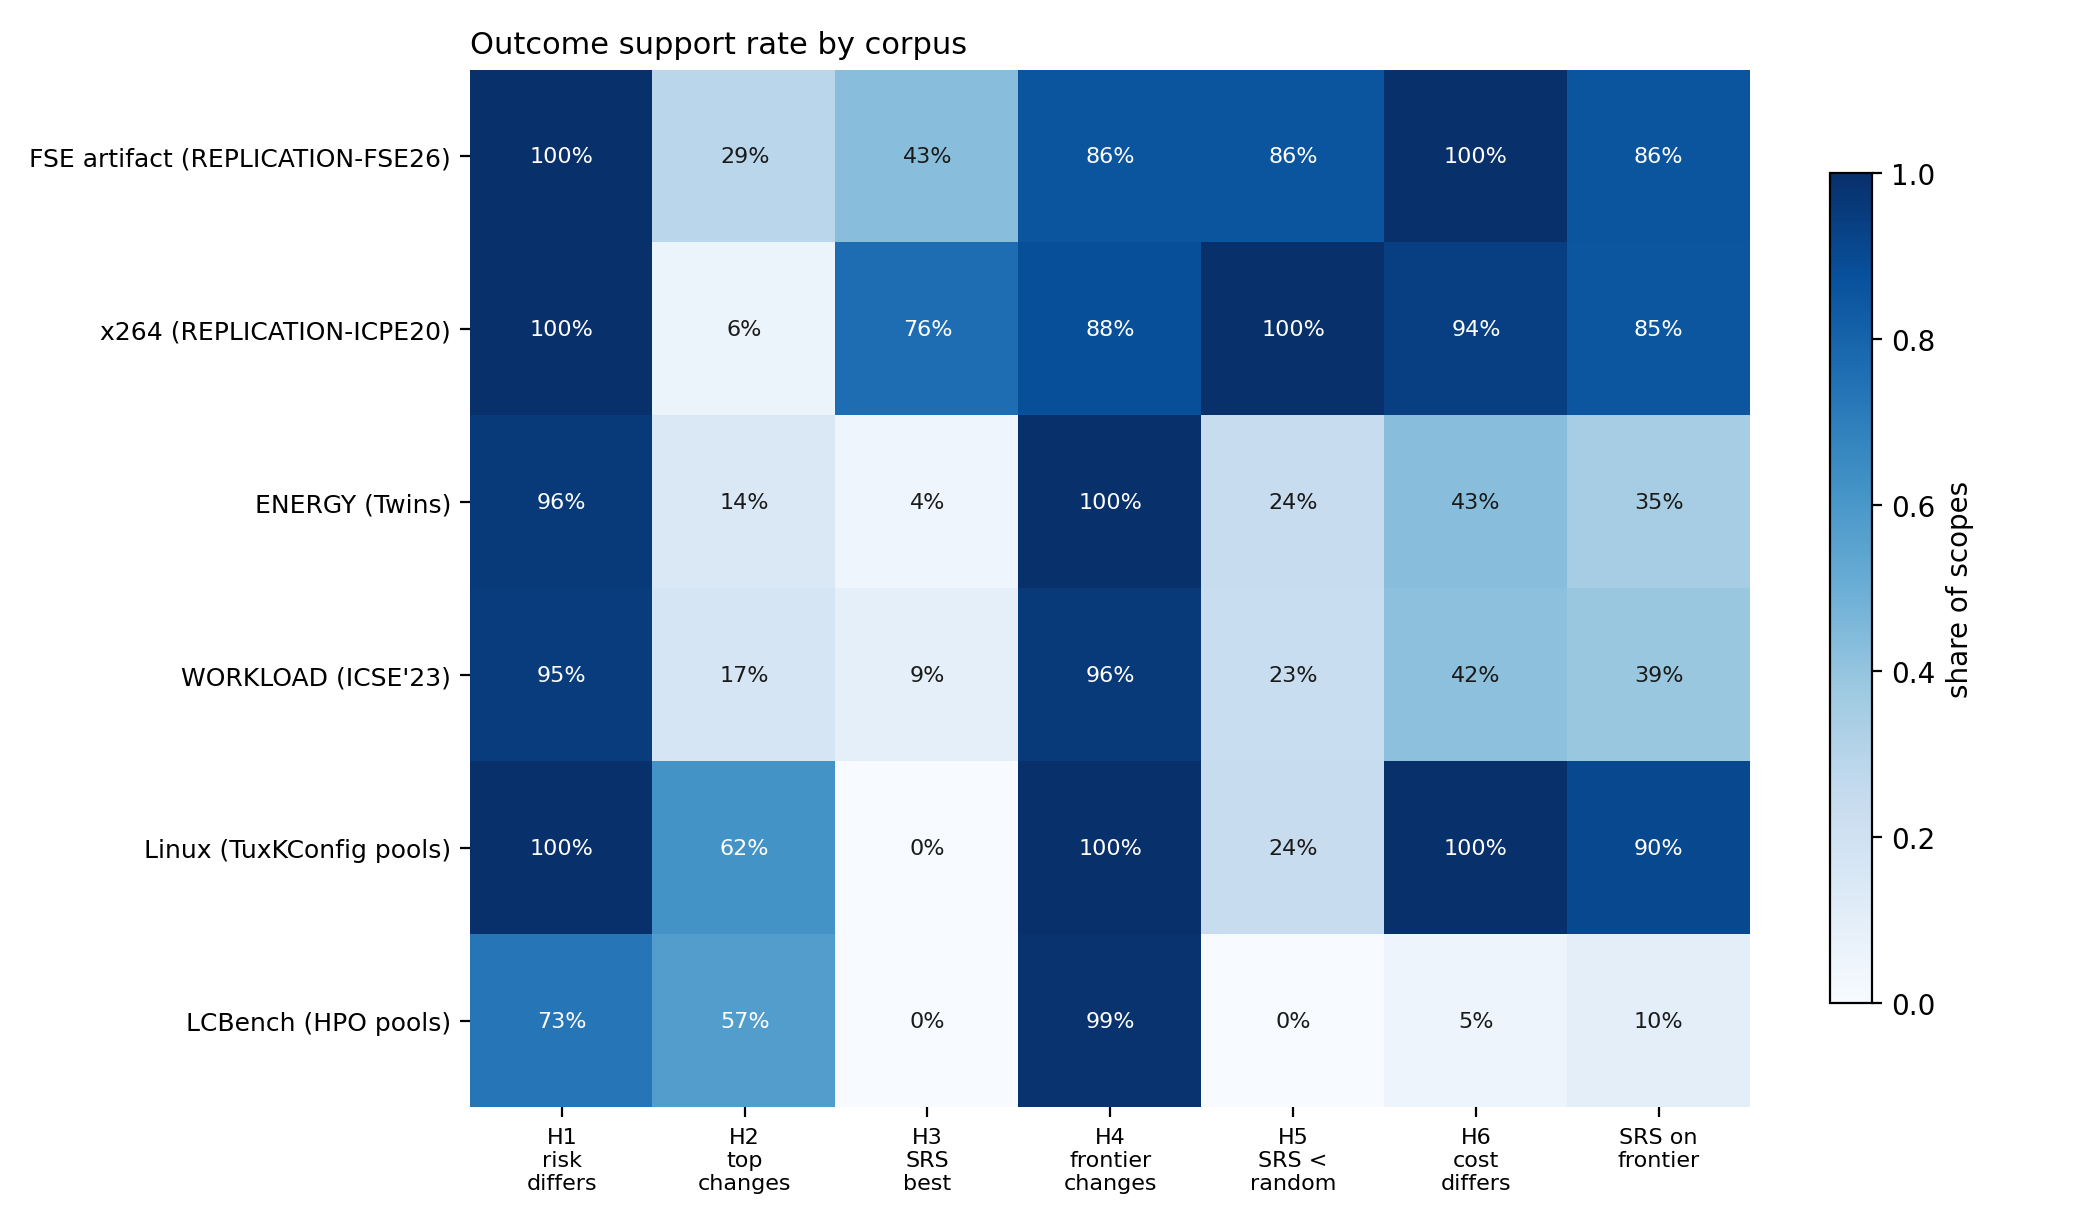
\includegraphics[width=.94\linewidth]{figures/fig_synthesis_heatmap.png}
  \caption{Outcome support rates by corpus (share of scopes; Linux row
  shows the full-protocol run). H1/H5/H6 are significance-based; H2--H4
  and frontier membership are decision rules
  (Section~\ref{sec:stats}).}
  \label{fig:heatmap}
\end{figure}

\subsection{RQ1.1: Discriminative power (C1)}

On the original artifact, all seven systems show significant differences
between the posterior-risk distributions of the five strategies,
reproducing C1 exactly. Figure~\ref{fig:polly} illustrates the
replication on Polly, the system the original paper singles out for
discussion, in the original paper's own visual idiom: per-strategy
posterior-risk distributions over 100 repetitions (left) and the
confidence discrepancy against the scenario-theoretic prior as the
accepted risk $\varepsilon$ varies (right). The strategies separate
cleanly---$t$-wise trades a deterministic, slightly higher risk for the
largest confidence gain at small $\varepsilon$, \srs{} and solver-based
sampling beat the prior, distance-based sampling falls below it. The
claim then generalizes to every corpus we add: 34/34 x264 contexts,
212/220 ENERGY scenarios, 341/359 WORKLOAD contexts, 21/21 Linux
release-level scopes, and 154/210 LCBench pools (144 after FDR
correction; the only corpus where correction moves the count). Overall,
posterior risk discriminates strategies in $\approx$95\% of 851
scopes---with no learner in the loop and across targets as different as
encoding time, energy, kernel size, and model accuracy.

\begin{figure}[t]
  \centering
  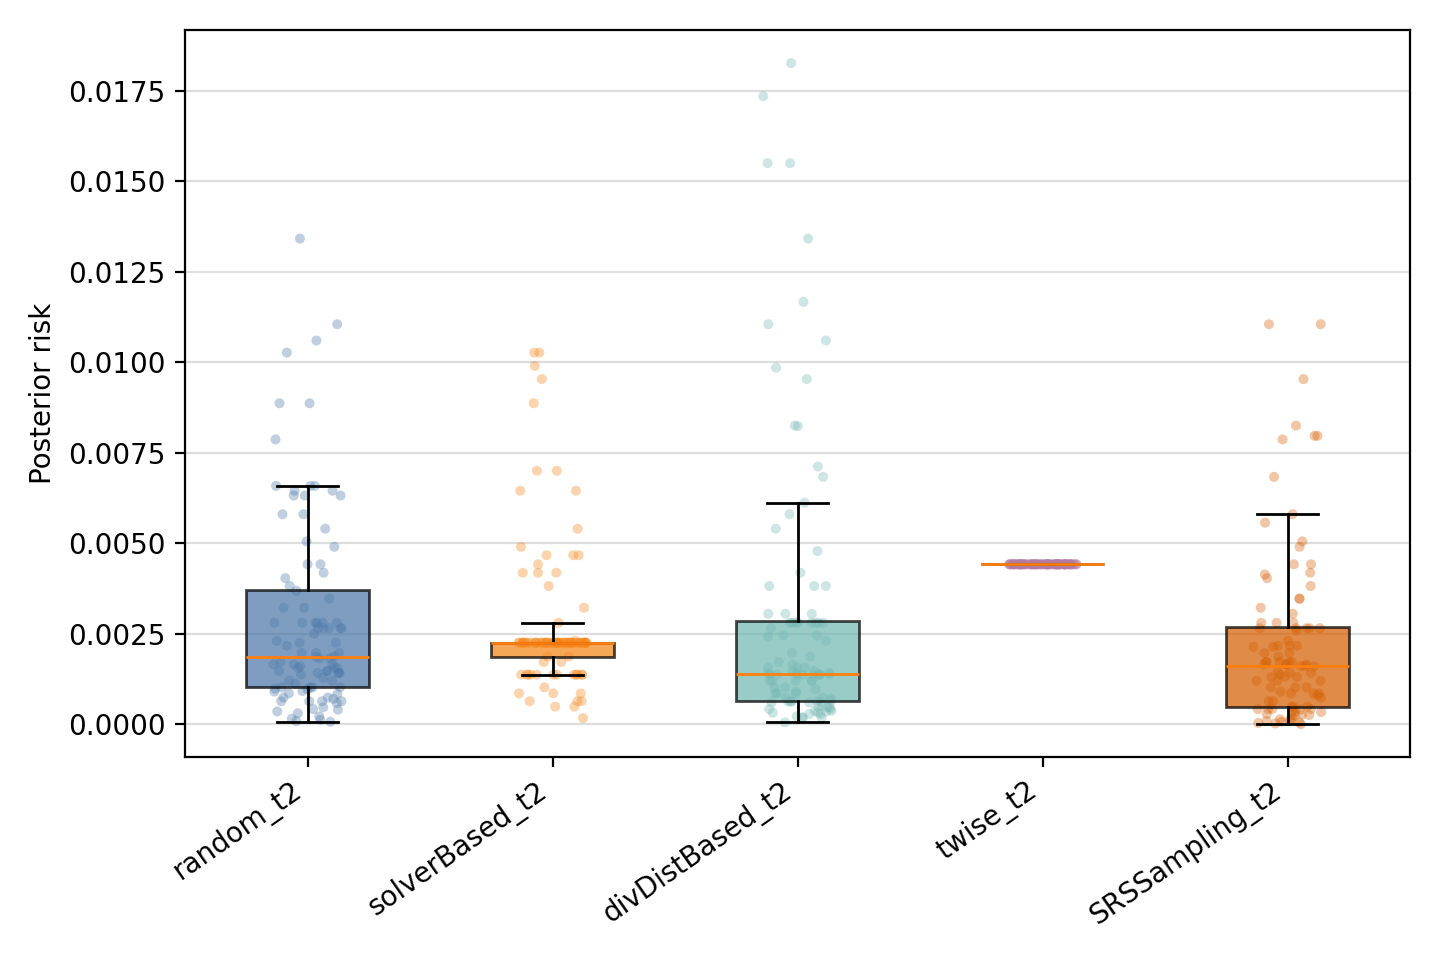
\includegraphics[width=.495\linewidth]{figures/fig_polly_risk.png}\hfill
  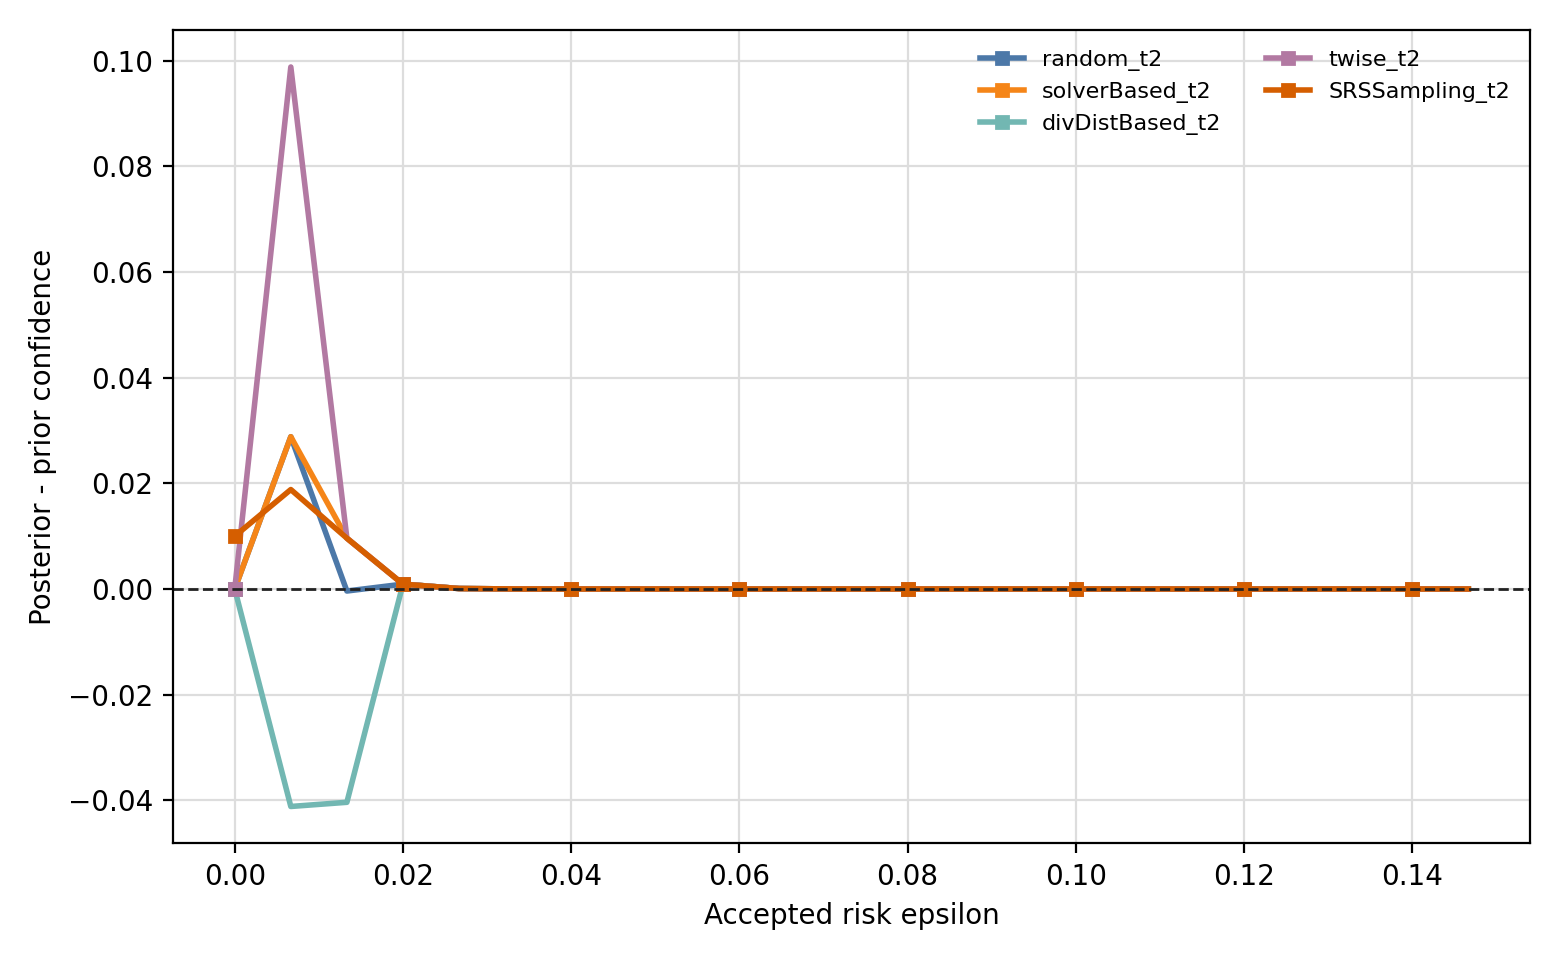
\includegraphics[width=.495\linewidth]{figures/fig_polly_confidence.png}
  \caption{Close replication on Polly (60{,}000 configurations, budget
  $t2=345$), in the visual idiom of \citet{weis2026risk}. Left:
  posterior-risk distributions per strategy (100 repetitions). Right:
  posterior minus prior confidence as a function of the accepted risk
  $\varepsilon$ (positive: better guarantees than the random-sampling
  prior at the same size).}
  \label{fig:polly}
\end{figure}

\finding{Finding 1 (C1 replicates and generalizes). Posterior risk and
confidence discriminate sampling strategies in $\approx$95\% of 851
scopes across six corpora, robust to FDR correction. The FSE~2026
evaluation framework is sound and portable.}

\subsection{RQ1.2: Budget scaling (C4)}

For each (context, strategy) pair we check whether median posterior risk
is non-increasing (and integrated confidence non-decreasing) along the
budget grid; Table~\ref{tab:scaling} reports the share of cells where
this holds. On configurable-software corpora the FSE expectation holds
broadly: 100\% of x264 cells, 98\% of Linux cells, 81\% of WORKLOAD and
76\% of ENERGY cells (the generated families use small budgets where
single-seed deterministic strategies can be non-monotone). For \srs{}
specifically, scaling is perfect (100\%) on \emph{all}
configurable-software corpora. On LCBench, however, monotonicity degrades
to 65\% of cells overall and 49\% for \srs: on
hyperparameter-optimization pools, growing the sample does not reliably
tighten \srs's bound, because its recursive restriction can lock onto
hyperparameter regions whose accuracy plateau differs from where the
pool's true optimum lies.

\begin{table}[t]
  \centering\small
  \caption{RQ1.2, budget scaling: share of (context, strategy) cells
  whose guarantees improve monotonically along the budget grid (median
  risk non-increasing; integrated confidence non-decreasing), for all
  strategies and for \srs{} alone. The FSE artifact runs a single budget
  level and is not applicable.}
  \label{tab:scaling}
  \begin{tabular}{@{}lrrrr@{}}
    \toprule
    & \multicolumn{2}{c}{All strategies} & \multicolumn{2}{c}{\srs} \\
    \cmidrule(lr){2-3}\cmidrule(l){4-5}
    Corpus & risk $\downarrow$ & conf.\ $\uparrow$ & risk $\downarrow$ & conf.\ $\uparrow$ \\
    \midrule
    x264 & 100\% & 100\% & 100\% & 100\% \\
    ENERGY & 76\% & 77\% & 100\% & 100\% \\
    WORKLOAD & 81\% & 81\% & 100\% & 100\% \\
    Linux & 98\% & 100\% & 100\% & 100\% \\
    LCBench & 65\% & 65\% & 49\% & 54\% \\
    \bottomrule
  \end{tabular}
\end{table}

\finding{Finding 2 (C4 replicates within the population, cracks outside).
Guarantees improve monotonically with sample size for \srs{} on every
configurable-software corpus (100\% of cells), but only in 49\% of
LCBench cells---the first boundary condition.}

\subsection{RQ1.3: \srs{} superiority (C2)}

On the original artifact, \srs{} is significantly better than uniform
random in 6/7 systems (H5), has the highest integrated confidence in 5/7,
and the lowest median risk in 4/7---consistent with the original
finding that \srs{} is the strongest, though not uniformly dominant,
strategy. On x264 the replication is even stronger: significantly better
than random in 34/34 contexts, best integrated confidence in 28/34.
x264's budgets are $t$-wise-scale (dozens to hundreds of samples),
matching the original protocol. Table~\ref{tab:ranks} summarizes the
fixed-size strategy ranking on both replication corpora: \srs{} is the
top-ranked strategy on both (mean rank 1.6 of 5, and 1.1 of 7), with
distance-based sampling a consistent second.

\begin{table}[t]
  \centering\small
  \caption{RQ1.3--1.4, fixed-size strategy ranking on the replication
  corpora: mean rank by median posterior risk across contexts at the
  $t2$ budget (1 = lowest risk). Strategies absent from a corpus are
  marked ---.}
  \label{tab:ranks}
  \begin{tabular}{@{}lrr@{}}
    \toprule
    Strategy & FSE artifact (of 5) & x264 (of 7) \\
    \midrule
    \srs & \textbf{1.6} & \textbf{1.1} \\
    Diversified distance-based & 2.3 & 2.9 \\
    Uniform random & 3.0 & 3.3 \\
    Distance-based & --- & 4.3 \\
    $t$-wise & 4.1 & 4.4 \\
    Henard's diversified & --- & 5.1 \\
    Solver-based & 3.7 & 6.1 \\
    \bottomrule
  \end{tabular}
\end{table}

The claim does not travel further. On the generated families at small
budgets ($n{=}8$--$64$), \srs{} is best in only 5--20\% of scopes and
beats random significantly in $\approx$19\% (FDR-corrected);
space-filling strategies (\diShe, \pairwise) dominate. On Linux, \srs{}
is \emph{never} the best strategy at fixed size (0/21) and beats random
in only 1/21 scopes after correction; on LCBench it is best by
integrated confidence in a single pool (1/210) and never by risk. Anticipating
Section~\ref{sec:rq2}: the equal-spend experiment shows this is chiefly a
\emph{budget} effect---\srs's advantage over random grows from 4\% of
ENERGY scopes at $n8$-scale budgets to 77\% at $n64$-scale
(Figure~\ref{fig:equalspend}B)---which reconciles its dominance at the
original protocol's larger budgets with its weakness at ours.

\finding{Finding 3 (C2 replicates where FSE tested it; it is
budget- and domain-dependent). \srs{} superiority replicates fully on the
original systems and on x264 (34/34), fades at small budgets on the
generated families, and vanishes on Linux and LCBench (best in at most 1
of 231 scopes). The advantage requires budget to amortize.}

\subsection{RQ1.4: Solver unreliability (C3)}

Solver-based sampling ranks near the bottom on both corpora where it
participates (Table~\ref{tab:ranks}): mean median-risk rank 3.7 of 5
strategies on the FSE artifact and clearly worst, 6.1 of 7, on x264. On
the FSE artifact only $t$-wise ranks lower by median risk---but
$t$-wise's deterministic sample yields zero risk variance and hence high
confidence at small tolerances, whereas solver-based sampling combines
mediocre risk with high variance, matching the original paper's
characterization of unreliable guarantees. Its samples, drawn from a SAT
solver's biased enumeration order, systematically miss the performance
extremes that bounds require, echoing prior findings on solver bias
\citep{plazar2019uniform}.

\finding{Finding 4 (C3 replicates). Plain solver-based sampling remains
the least reliable strategy for guarantees on both corpora that include
it.}

\subsection{\rqone{} answer}

All four FSE claims replicate on the original artifact under exact data
reuse, and the framework-level claims (C1, C3) replicate on every
applicable corpus. The strategy-level claims (C2, C4) replicate within
the population the original study sampled from---configurable software at
$t$-wise-scale budgets---and degrade predictably outside it. No claim
reverses on the original systems. In replication terms: a successful
close replication, and a conceptual replication that maps the claims'
boundary conditions rather than refuting them.

\section{\rqtwo: Do the Metrics Survive Measured Cost?}
\label{sec:rq2}

We now hold the metrics fixed and change one construct: the budget axis,
from sample count to measured acquisition cost
(Section~\ref{sec:costargument}).

\subsection{RQ2.1--2.2: Cost heterogeneity and the calibration of size as
a proxy}
\label{sec:rq21}

A fixed sample size is not a fixed measured effort. Within-system
per-configuration costs vary by up to a coefficient of variation of 1.42
and a $p90/p10$ ratio of 47.9 (BerkeleyDB-C) on the FSE artifact alone.
Consequently, the calibration ratio $\%cost/\%n$ of actual samples---1.0
when a sample is cost-representative---is centered near 1.0 in every
corpus but with heavy tails: 0.19--3.11 across FSE-artifact cells,
0.03--7.05 on ENERGY, 0.09--2.77 on WORKLOAD, 0.04--2.48 on LCBench,
0.64--2.57 on Linux, and 0.62--1.43 on x264
(Figure~\ref{fig:calibration}). In other words, sample size is an
approximately \emph{unbiased} but \emph{high-variance} proxy for
measurement effort: two strategies that both acquire $n$ configurations
can differ in actual spend by a factor of two to thirty, and the
direction of the deviation is strategy-systematic (e.g., \srs{} leans
expensive on Linux in 21/21 scopes, H6; \pilotcost{} leans cheap by
construction).

\begin{figure}[t]
  \centering
  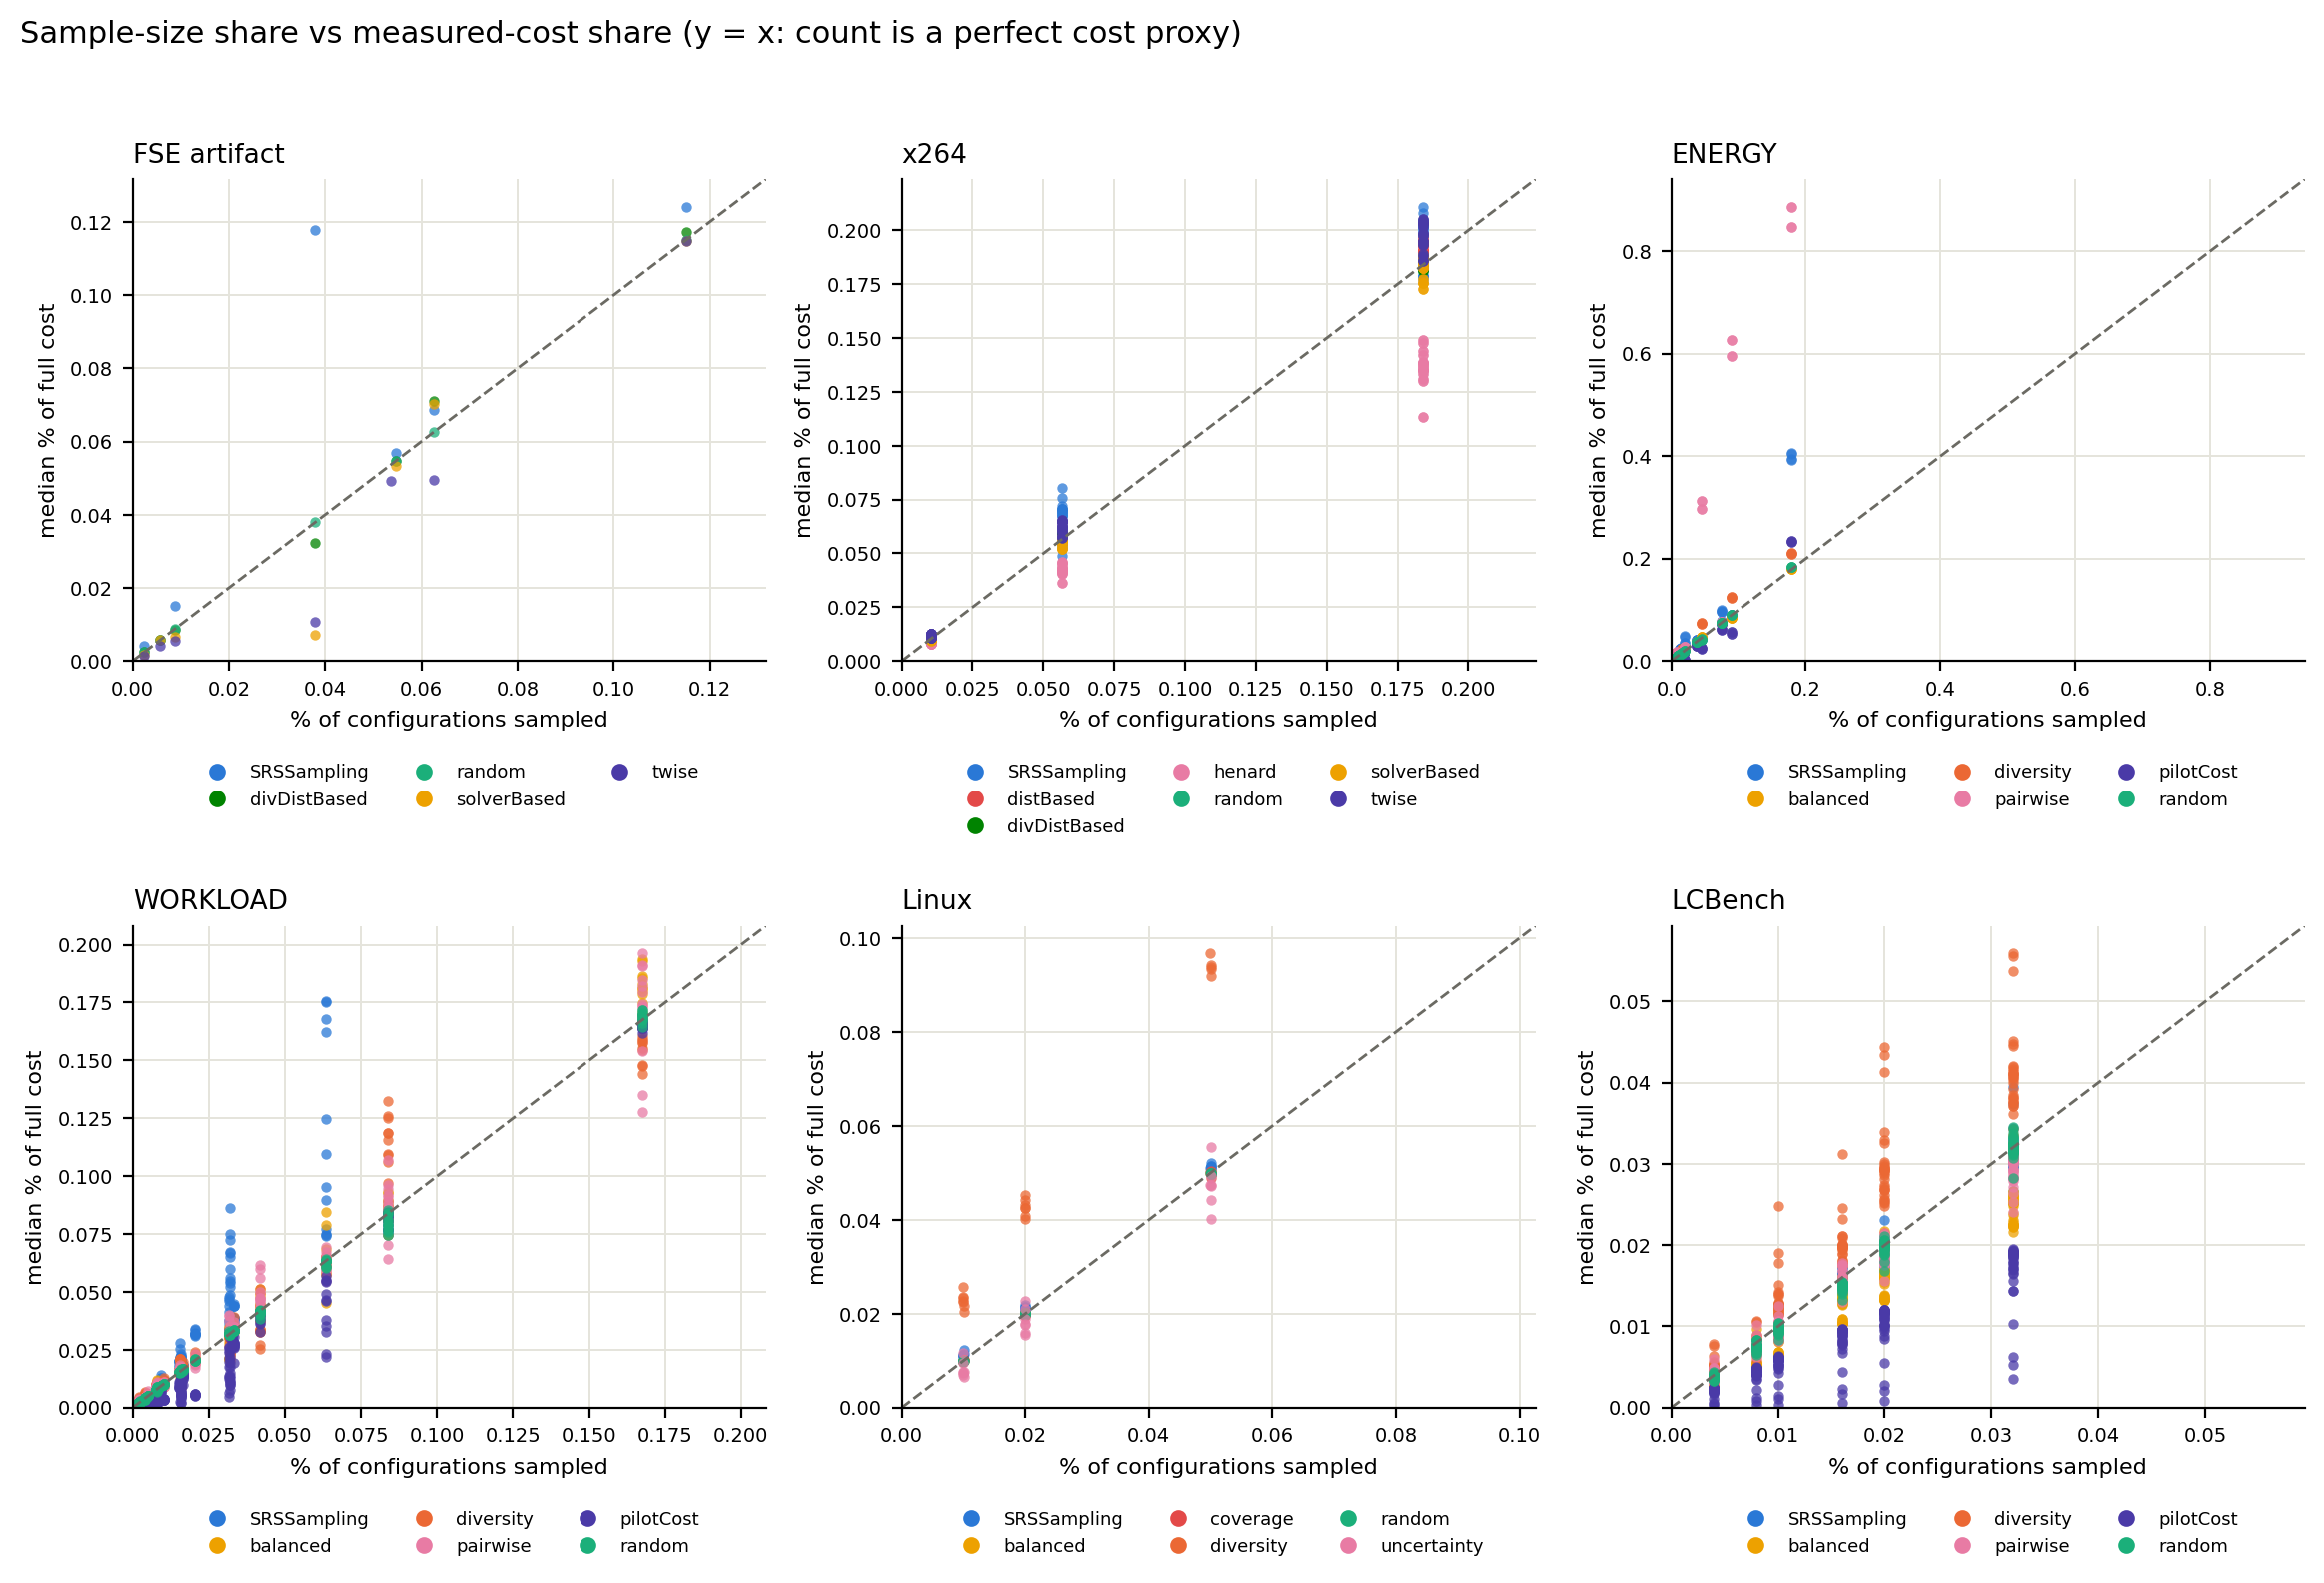
\includegraphics[width=.92\linewidth]{figures/fig_calibration_pct_n_vs_pct_cost.png}
  \caption{Share of configurations sampled versus share of total
  measurement cost, per strategy and budget level (medians across runs).
  On the $y{=}x$ diagonal, sample size is a perfect cost proxy.}
  \label{fig:calibration}
\end{figure}

\finding{Finding 5. Sample size is an unbiased but high-variance proxy
for acquisition cost: same-size samples differ in measured spend by up to
an order of magnitude, and the deviations are strategy-systematic---a
construct-validity gap for any budgeted strategy comparison.}

\subsection{RQ2.3: Decision impact}
\label{sec:rq23}

Does the proxy error matter for decisions? Two decision artifacts can
change when the budget axis switches from $n$ to measured cost: the
single top recommendation (highest $\omega$), and the Pareto frontier
over (integrated confidence, budget)---the set of non-dominated
(strategy, budget) choices a practitioner should consider.
Table~\ref{tab:impact} and Figure~\ref{fig:impact} give the counts.

\begin{table}[t]
  \centering\small
  \caption{\rqtwo{} decision impact per corpus: scopes where the top
  recommendation (H2) and the Pareto frontier (H4) differ between the
  size axis and the measured-cost axis.}
  \label{tab:impact}
  \begin{tabular}{@{}lrrr@{}}
    \toprule
    Corpus & Scopes & Top changes (H2) & Frontier changes (H4) \\
    \midrule
    FSE artifact & 7 & 2 (29\%) & 6 (86\%) \\
    x264 & 34 & 2 (6\%) & 30 (88\%) \\
    ENERGY & 220 & 31 (14\%) & 220 (100\%) \\
    WORKLOAD & 359 & 61 (17\%) & 346 (96\%) \\
    Linux & 21 & 13 (62\%) & 21 (100\%) \\
    LCBench & 210 & 120 (57\%) & 207 (99\%) \\
    \midrule
    Total & 851 & 229 (27\%) & \textbf{830 (97.5\%)} \\
    \bottomrule
  \end{tabular}
\end{table}

\begin{figure}[t]
  \centering
  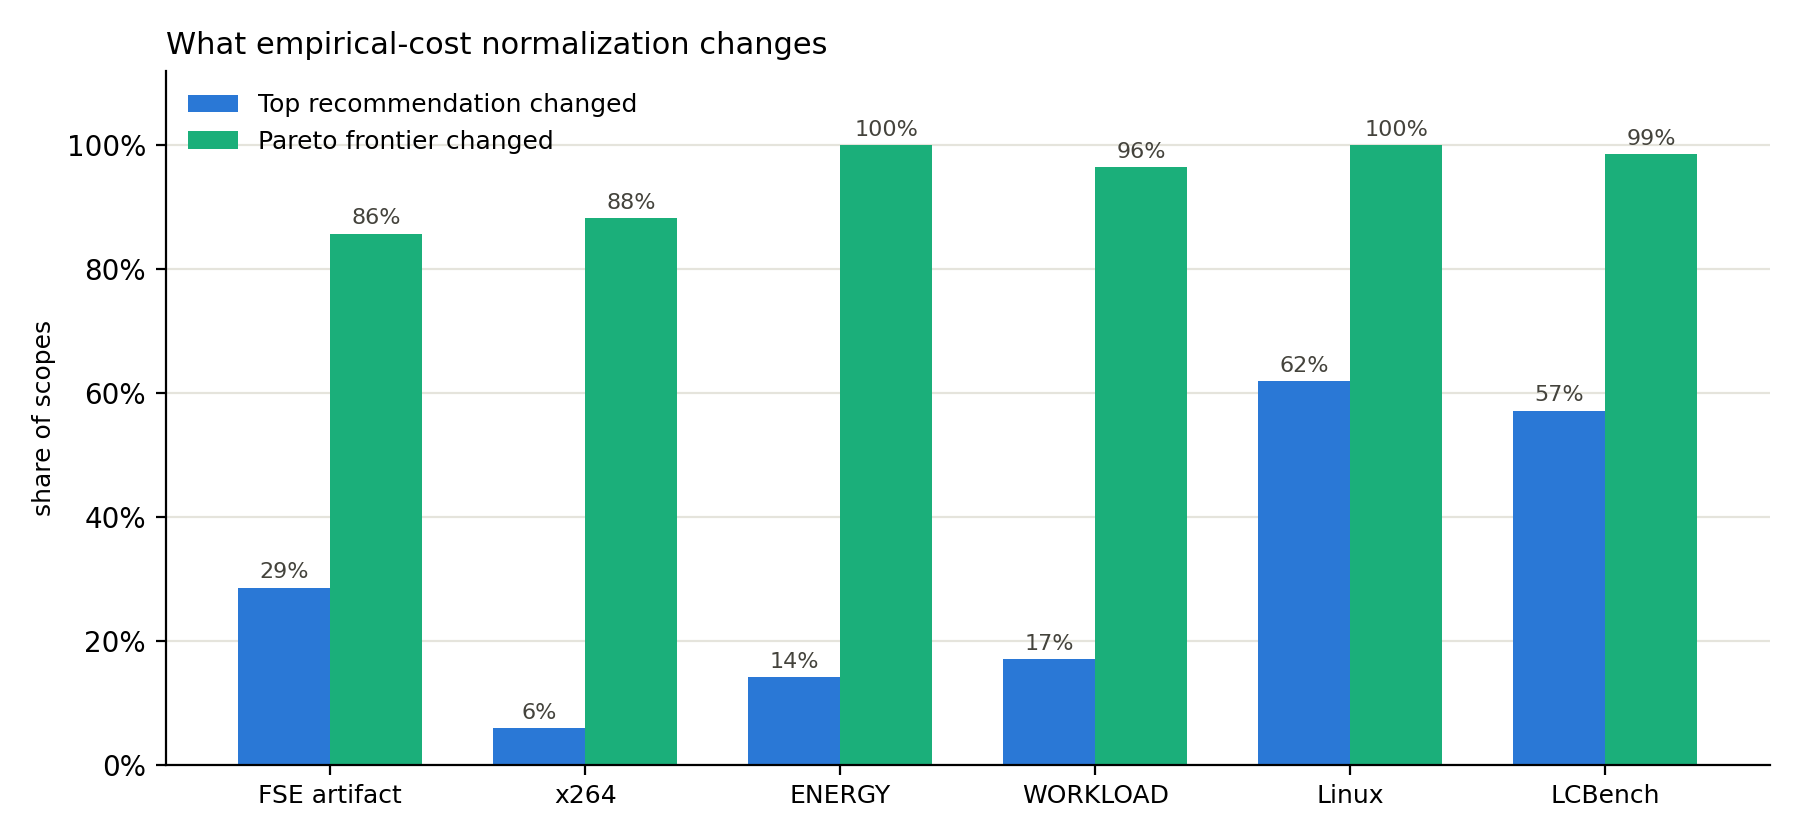
\includegraphics[width=.85\linewidth]{figures/fig_cost_normalization_impact.png}
  \caption{What switching the budget axis changes, per corpus: the single
  top recommendation versus the Pareto frontier of defensible choices.}
  \label{fig:impact}
\end{figure}

The frontier result is the most robust effect in our data: in 830 of 851
scopes (97.5\%), the set of guarantee/cost-efficient choices under
measured cost differs from the set under sample count, and not
marginally: the median Jaccard overlap between the two frontiers is
0.14--0.33 depending on the corpus. The top-1 recommendation is more
stable and strongly corpus-dependent---from 6\% of x264 contexts to 62\%
on Linux: the Pareto-level effect is the robust one, single-winner flips
the secondary one.

Even on the original FSE artifact, re-indexing by the artifact's own
runtime measurements changes the frontier in 6/7 systems.
Table~\ref{tab:fseartifact} gives the per-system view: cost
heterogeneity (columns 3--4) is a property of the system, and where it
is large (7z, BerkeleyDB-C), the size-indexed and cost-indexed winners
diverge---\srs{} wins both axes only on the three systems whose samples
happen to be nearly cost-representative. The frontier overlap (last
column) is below $0.5$ on six of seven systems.

\begin{table}[t]
  \centering\small
  \caption{Per-system decisions on the original FSE artifact at the $t2$
  budget. CV: coefficient of variation of per-configuration cost;
  $p90/p10$: cost dispersion; best by size/cost: winner by integrated
  confidence discrepancy under each budget axis; $J$: Jaccard overlap of
  the two Pareto frontiers.}
  \label{tab:fseartifact}
  \setlength{\tabcolsep}{4.5pt}
  \begin{tabular}{@{}lrrrllr@{}}
    \toprule
    System & $|\mathcal{V}|$ & Cost CV & $p90/p10$ & Best by size & Best by cost & $J$ \\
    \midrule
    7z & 68{,}640 & 1.19 & 10.1 & \srs & $t$-wise & 0.50 \\
    BerkeleyDB-C & 2{,}560 & 1.42 & 47.9 & \srs & \randomS & 0.20 \\
    Dune & 2{,}304 & 0.34 & 1.8 & \srs & \srs & 0.25 \\
    Hipacc & 13{,}485 & 0.44 & 2.6 & distance & distance & 0.25 \\
    JavaGC & 193{,}536 & 1.02 & 7.8 & \srs & \srs & 0.33 \\
    LLVM & 1{,}024 & 0.07 & 1.2 & distance & distance & 1.00 \\
    Polly & 60{,}000 & 0.24 & 2.1 & \srs & \srs & 0.20 \\
    \bottomrule
  \end{tabular}
\end{table}

\finding{Finding 6. Re-indexing guarantees by measured cost changes the
Pareto frontier of defensible (strategy, budget) choices in 97.5\% of 851
scopes---including 6/7 original FSE systems---while the single top pick
changes in 27\%. Sample-size budgets systematically misrepresent the
decision surface a cost-aware practitioner faces.}

\subsection{RQ2.4: Cost-normalized recommendation}
\label{sec:rq24}

Which strategy is best per unit of measured cost, by
$\omega_{\mathrm{cost}}$? Table~\ref{tab:winners} counts the
cost-normalized winners per corpus. \srs{} remains the winner where it
also won at fixed size---26/34 x264 contexts, 3/7 FSE-artifact
systems---but nowhere else: 9/220 ENERGY, 31/359 WORKLOAD, 0/21 Linux,
0/210 LCBench (Figure~\ref{fig:srsstatus}). On the small-budget families
the space-filling strategies dominate the cost-normalized picks
(\diShe{} 108 and \pairwise{} 74 of 220 on ENERGY; \pairwise{} 155 and
\diShe{} 108 of 359 on WORKLOAD), and on LCBench even the cost-aware
\pilotcost{} takes a quarter of the scopes (54/210)---a first hint of the
coupling mechanism that Section~\ref{sec:rq25} isolates.

\begin{table}[t]
  \centering\small
  \caption{RQ2.4, cost-normalized winners: how often each strategy has
  the highest integrated-confidence discrepancy against the cost-indexed
  prior ($\omega_{\mathrm{cost}}$), per corpus (winners with at least
  two scopes shown).}
  \label{tab:winners}
  \setlength{\tabcolsep}{5pt}
  \begin{tabular}{@{}lrl@{}}
    \toprule
    Corpus & Scopes & Cost-normalized winners (scopes won) \\
    \midrule
    FSE artifact & 7 & \srs{} (3), distance-based (2), $t$-wise (1), \randomS{} (1) \\
    x264 & 34 & \srs{} (26), Henard's (5), distance-based (3) \\
    ENERGY & 220 & \diShe{} (108), \pairwise{} (74), \balanced{} (20), \srs{} (9) \\
    WORKLOAD & 359 & \pairwise{} (155), \diShe{} (108), \balanced{} (48), \srs{} (31) \\
    Linux & 21 & \diShe{} (19), \textsf{uncertainty} (1), \balanced{} (1) \\
    LCBench & 210 & \diShe{} (69), \balanced{} (62), \pilotcost{} (54), \pairwise{} (25) \\
    \bottomrule
  \end{tabular}
\end{table}

Linux crystallizes the distinction between \emph{winning} and
\emph{being worth considering}. At full statistical power (100 seeds),
\srs{} is never the best cost-normalized strategy (0/21), its acquisition
cost differs significantly from random's in 21/21 scopes---it buys
systematically more expensive kernels---and yet it sits \emph{on} the
empirical guarantee/cost frontier in 19/21 scopes
(Figure~\ref{fig:frontiers} illustrates the three regimes: \srs{} best,
\srs{} on the frontier without winning, \srs{} dominated). \srs{} buys
real guarantee quality at a real cost premium; the cost-indexed analysis
does not dismiss the strategy, it \emph{prices} it.
Figure~\ref{fig:keysystems} shows two key extension systems in detail.
On the Linux~4.13 pool (92{,}562 kernels, 2\% budget level), \srs{} is
the archetypal frontier point: essentially the best confidence available
at its spend, while \diShe{} buys the final $5\cdot10^{-4}$ of
integrated confidence at more than twice the cost. On the lrzip energy
scenario, \srs{} is dominated---\diShe{} achieves more confidence at
half the spend---and the cost-aware \pilotcost{} is by far the cheapest
strategy yet delivers drastically weaker guarantees, previewing the
equal-spend mechanism of Section~\ref{sec:rq25}.

\begin{figure}[t]
  \centering
  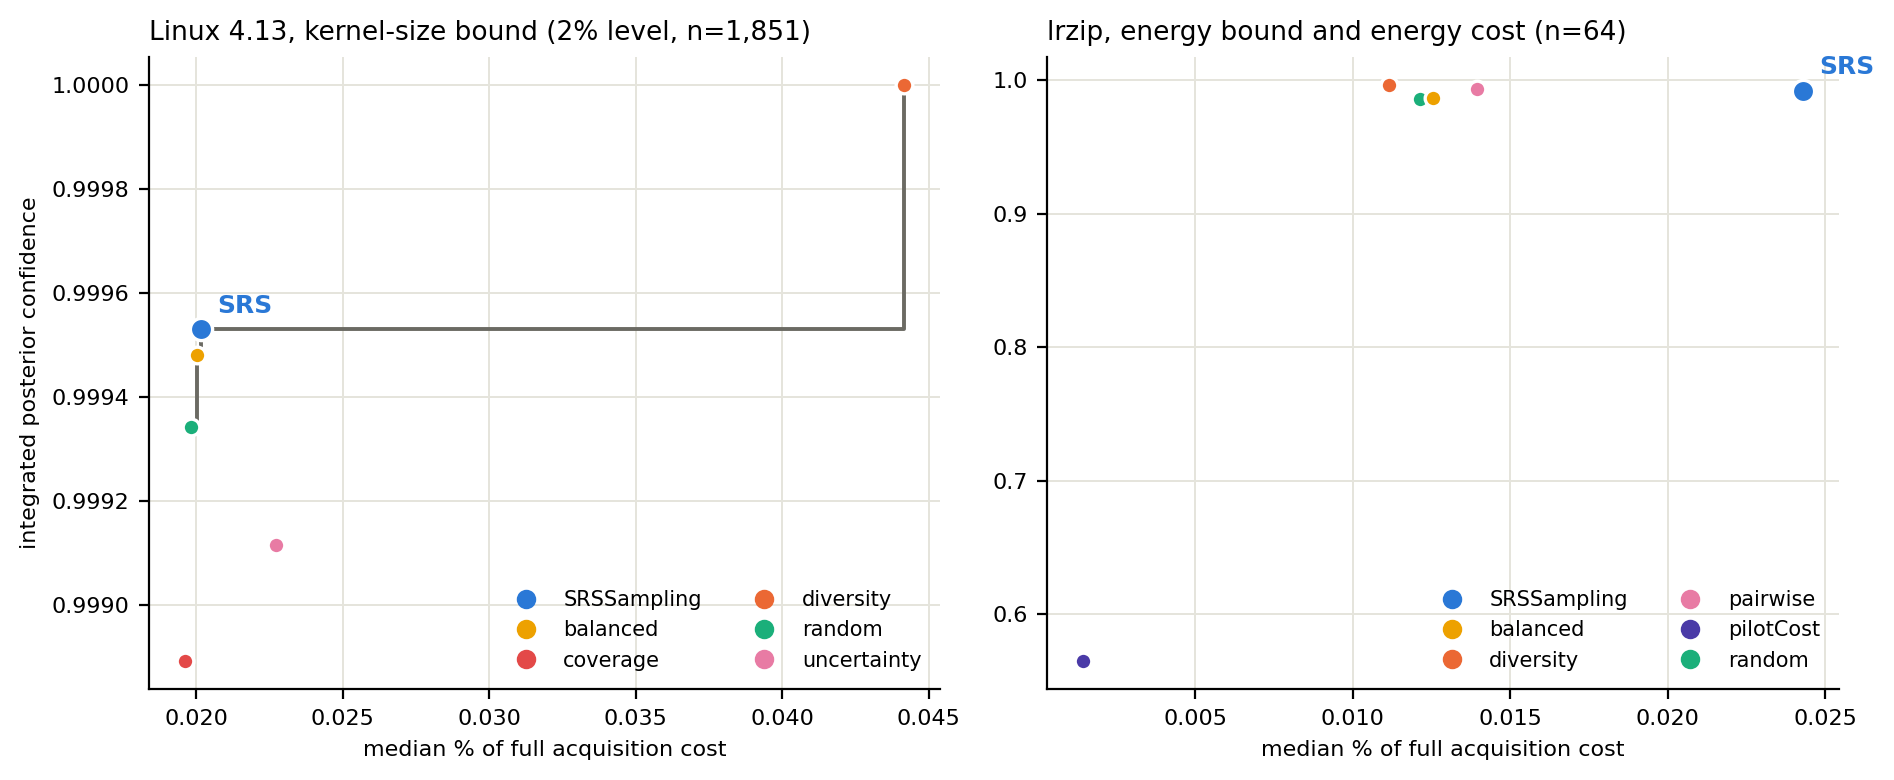
\includegraphics[width=\linewidth]{figures/fig_key_systems.png}
  \caption{Guarantee/cost view of two key extension systems at one
  budget level each (points: strategies; line: empirical cost/confidence
  Pareto frontier; median integrated confidence versus median share of
  full acquisition cost). Left: Linux~4.13, kernel-size bound
  (pool-relative; note the narrow confidence range). Right: lrzip with
  energy as both target and cost.}
  \label{fig:keysystems}
\end{figure}

\begin{figure}[t]
  \centering
  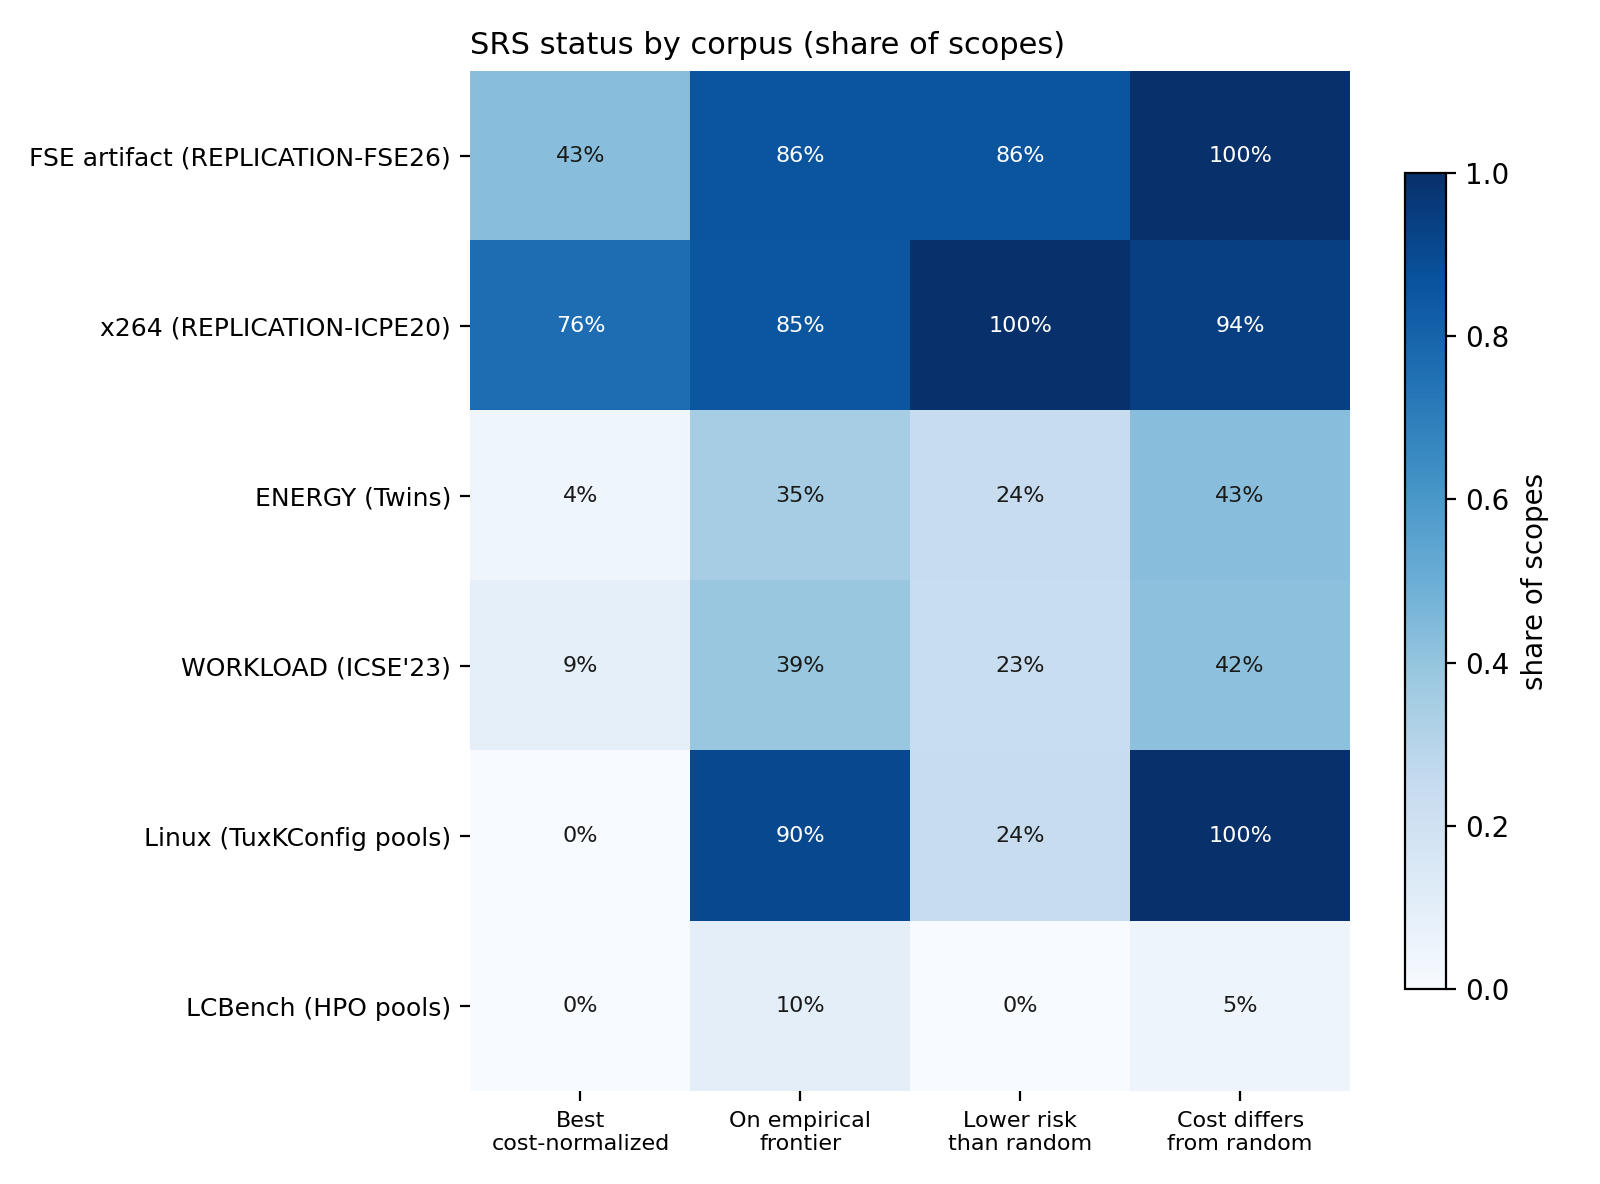
\includegraphics[width=.8\linewidth]{figures/fig_srs_status_matrix.png}
  \caption{\srs{} status per corpus under measured cost (share of
  scopes).}
  \label{fig:srsstatus}
\end{figure}

\begin{figure}[t]
  \centering
  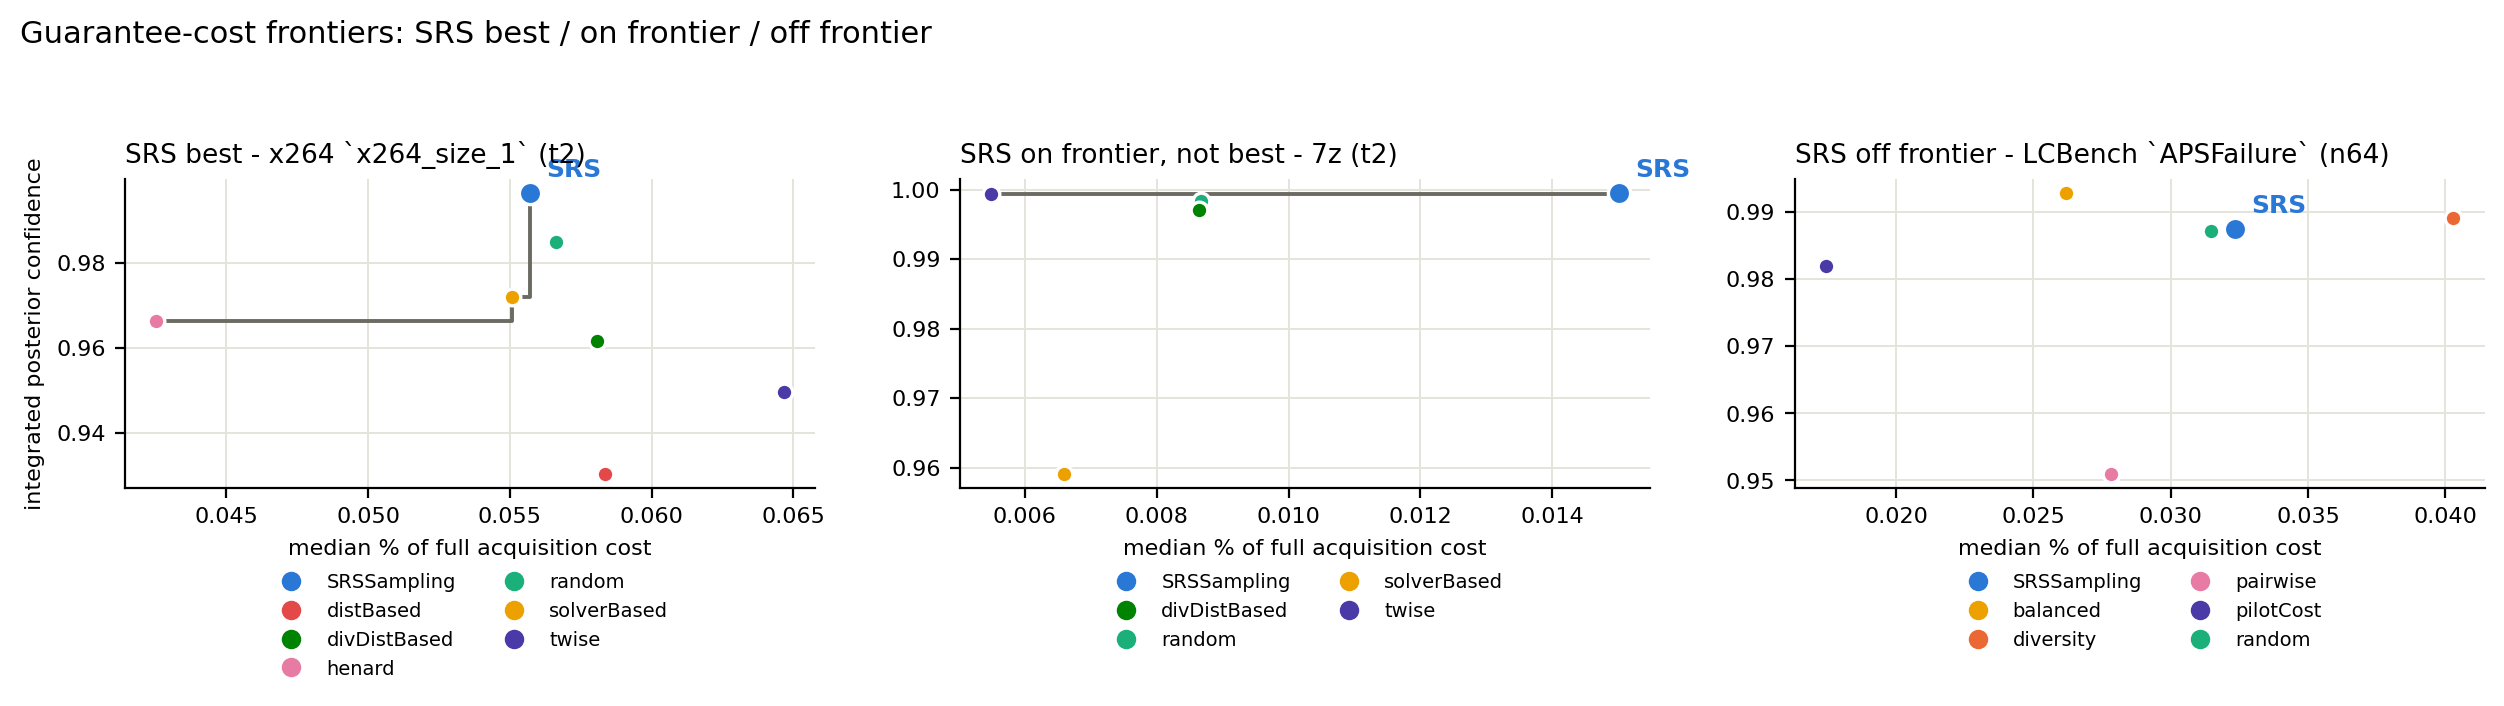
\includegraphics[width=\linewidth]{figures/fig_frontiers_representative.png}
  \caption{Representative guarantee/cost frontiers (points: strategies at
  one budget level; line: empirical cost/confidence Pareto frontier).
  Left: \srs{} best (x264). Middle: \srs{} on the frontier but not best
  (7z, FSE artifact). Right: \srs{} dominated (LCBench pool).}
  \label{fig:frontiers}
\end{figure}

\finding{Finding 7. Under cost normalization \srs{} keeps its crown only
on the replication corpora (x264 26/34; FSE artifact 3/7). On Linux it is
never best yet frontier-competitive in 90\% of scopes with an
always-significant cost premium: cost-indexing prices strategies rather
than dismissing them.}

\subsection{RQ2.5: Equal spend, and the mechanism}
\label{sec:rq25}

The $\omega_{\mathrm{cost}}$ handicap is a counterfactual. The
equal-spend protocol (Section~\ref{sec:equalspend}) makes it literal:
every strategy spends the same measured budget $B$ and buys however many
configurations $B$ affords. This is exactly the setting that cost-aware
strategy design targets \citep{sarkar2015cost,nair2017bad}, and
\pilotcost{} is built for it: it converts a fixed spend into
substantially more measured configurations than any cost-blind strategy.

\begin{figure}[t]
  \centering
  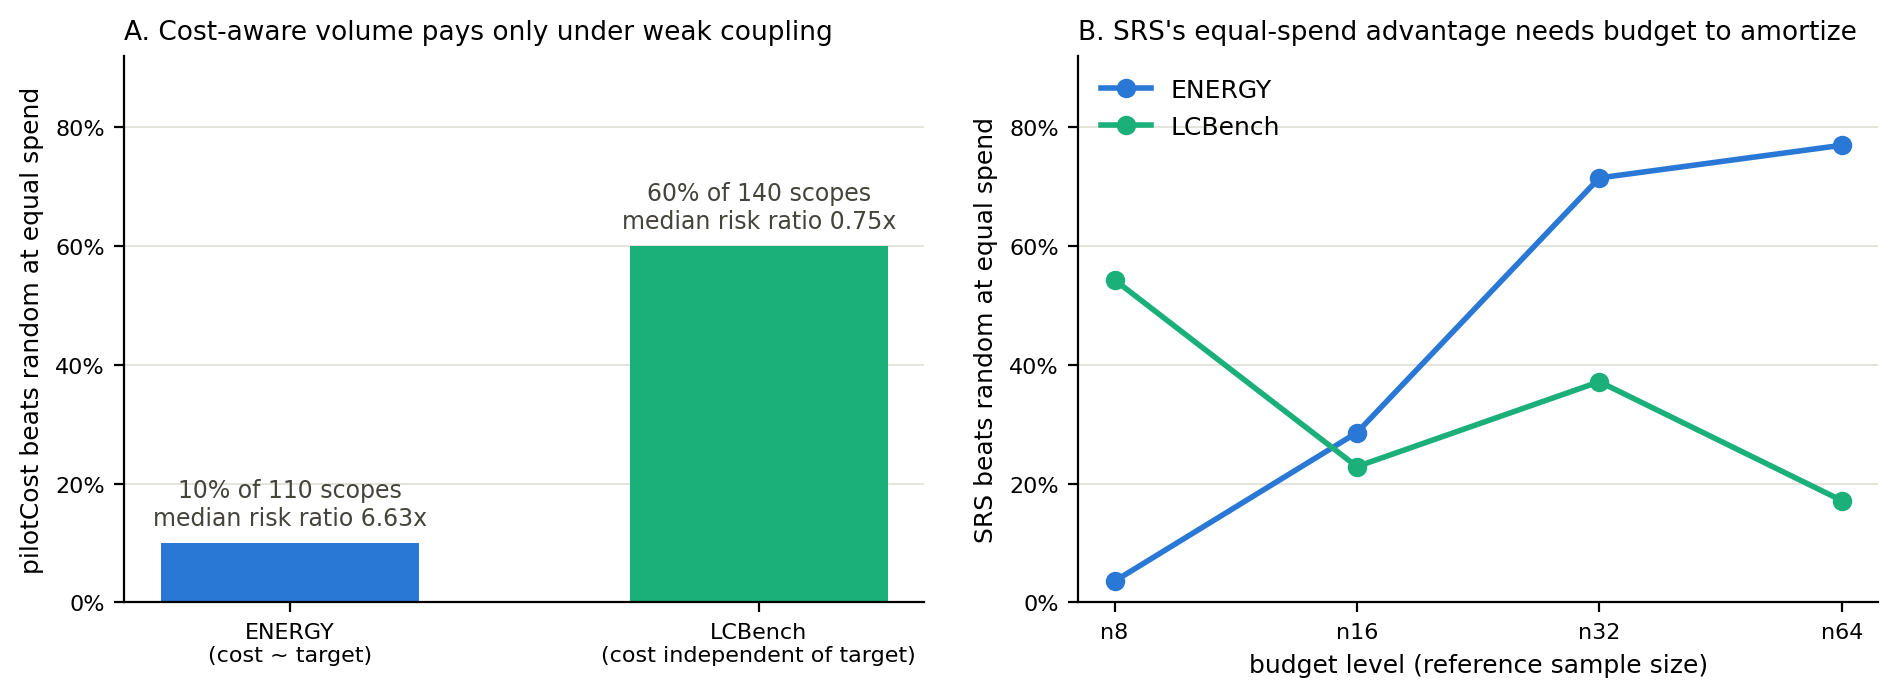
\includegraphics[width=\linewidth]{figures/fig_equal_spend.png}
  \caption{Equal-measured-spend experiments. (A)~\pilotcost{} versus
  uniform random across the coupling spectrum: share of scopes where
  \pilotcost's realized bound risk is lower, with the median risk ratio.
  (B)~Share of scopes where \srs{} beats random at equal spend, by budget
  level.}
  \label{fig:equalspend}
\end{figure}

For guarantees, the picture splits by \emph{cost--target coupling}
(Figure~\ref{fig:equalspend}A). On ENERGY, where cost (energy or
runtime) is strongly correlated with the bounded target, \pilotcost{}
converts its budget into $2.05\times$ more configurations (median; up to
$5\times$ on cost-heterogeneous systems)---and still loses: it beats
random in 11/110 scopes, with a median realized risk $6.6\times$
\emph{worse}. The information that a worst-case bound needs lives in the
expensive tail of the cost distribution, precisely the region a
cost-avoiding strategy refuses to buy; no volume of cheap configurations
substitutes for it. On LCBench, where training runtime and final accuracy
are only weakly coupled, the verdict flips: with a $1.66\times$ volume
advantage, \pilotcost{} beats random in 84/140 scopes with a median risk
ratio of 0.75. Cost-aware volume pays exactly when the outcome-relevant
information is \emph{not} concentrated in the expensive tail.

Table~\ref{tab:equalspend} summarizes both experiments.

\begin{table}[t]
  \centering\small
  \caption{RQ2.5, equal measured spend: every strategy buys the sample
  size the budget $B$ affords. Volume: \pilotcost's median affordable-$n$
  multiplier over \randomS. Risk ratio: median of
  \pilotcost's realized bound risk over \randomS's.}
  \label{tab:equalspend}
  \setlength{\tabcolsep}{4.5pt}
  \begin{tabular}{@{}lrrrrrl@{}}
    \toprule
    & & \multicolumn{3}{c}{\pilotcost{} vs.\ \randomS} & & \\
    \cmidrule(lr){3-5}
    Family & Scopes & volume & beats & risk ratio & \srs{} beats \randomS & Top winner \\
    \midrule
    ENERGY (cost $\sim$ target) & 110 & $2.05\times$ & 11 (10\%) & $6.6\times$ & 49 (45\%) & \diShe{} (47) \\
    LCBench (cost $\perp$ target) & 140 & $1.66\times$ & 84 (60\%) & $0.75\times$ & 46 (33\%) & \diShe{} (80) \\
    \bottomrule
  \end{tabular}
\end{table}

The same experiment resolves the \srs{} budget question raised in
\rqone{} (Figure~\ref{fig:equalspend}B). On ENERGY, \srs's equal-spend
win rate over random climbs from 1/28 scopes at $n8$-scale budgets to
20/26 at $n64$-scale: its recursive space restriction needs enough batches
to pay for itself, which is why it dominates at the original study's
$t$-wise-scale budgets and disappears at small ones. On LCBench the
gradient runs the other way (54\% down to 17\%): with cost and target
decoupled, random's cheap volume catches up with the pool's extremes
faster than \srs's guided-but-expensive search. Across both experiments
the overall winner is unchanged---\diShe{} wins 47/110 and 80/140
scopes---so the equal-spend protocol and the
$\omega_{\mathrm{cost}}$ handicap agree on every corpus-level conclusion,
ruling out the methodology as the explanation.

\finding{Finding 8. At literal equal spend, cost-effectiveness is
governed by cost--target coupling and budget amortization: the cost-aware
\pilotcost{} flips from $6.6\times$-worse to better-than-random as
coupling weakens, and \srs's advantage grows from 4\% to 77\% of scopes
as the budget grows. ``Cost-effective'' is a property of the (strategy,
outcome, coupling) triple---not of a strategy alone.}

\subsection{\rqtwo{} answer}

The FSE metrics themselves survive the re-indexing unchanged: posterior
risk, confidence, and $\omega$ are as computable and discriminative
against a cost-indexed baseline as against a size-indexed one. What does
not survive is the invariance of the \emph{decisions} they support. The
frontier of defensible choices moves in 97.5\% of scopes; the
cost-normalized winner is \srs{} only within the original population; and
equal-spend testing shows the governing mechanisms to be properties the
sample-size abstraction cannot express---where cost lives relative to the
target, and how much budget a strategy needs before its guidance
amortizes.

\section{Discussion}
\label{sec:discussion}

\subsection{What kind of replication outcome is this?}

Our results are simultaneously a strong confirmation and a strong
qualification of \citet{weis2026risk}, and it is worth being precise
about which is which. Everything the original paper \emph{measures}
replicates: the guarantee framework discriminates strategies wherever we
take it, its statistical behavior is robust to FDR correction, and on the
original artifact---with the authors' own strategy samples---every
headline claim reproduces under an independent reimplementation. What
does not generalize is the \emph{decision layer} built on top: which
strategy to recommend, and at what budget. Both turned out to be
population-relative in ways the original single-corpus,
single-budget-scale design could not observe. This is precisely the
epistemic value that replication studies are supposed to add
\citep{shull2008role,gomez2014understanding}: not a verdict on the
original, but a map of where its conclusions hold.

\subsection{The triple: strategy, outcome, coupling}

The equal-spend experiments turn the cost argument from an accounting
observation into a mechanism. In learning-oriented settings, cost-aware
sampling is defensible: cheap configurations carry option-effect
information a learner can use, so buying more of them per unit spend can
be a real gain \citep{sarkar2015cost,nair2017bad}. For worst-case bounds
the same policy can be self-defeating, because a bound is an extreme
order statistic: only samples near the top of the target distribution
move it, and when acquisition cost correlates with the target, those are
exactly the configurations a cost-avoider skips. The \pilotcost{} flip
(risk ratio $6.6\times$ worse under strong coupling, $0.75\times$ under
weak) is the cleanest demonstration we know of that
\emph{cost-effectiveness is not a strategy property}: the same strategy,
under the same equal-spend accounting, is the right choice for one
(outcome, coupling) pair and the wrong one for another. Evaluations that
report a single ``best strategy per dollar'' without fixing the outcome
and characterizing the coupling are underdetermined.

The \srs{} budget gradient is the second face of the same coin. \srs{}
spends its early budget learning \emph{where} to sample; that investment
amortizes only if enough budget remains to exploit it. At the original
study's $t$-wise-scale budgets it does; at $n{=}8$--$64$ it does not.
Neither our small-budget result nor the original large-budget result is
wrong---they sit at different points of an amortization curve that
Figure~\ref{fig:equalspend}B makes explicit.

\subsection{Implications}

\emph{For practitioners.} First, budget in measured units, not samples:
the frontier of defensible choices moves in 97.5\% of scopes when the
axis switches, and same-size samples can differ in real spend by an order
of magnitude. Second, think in frontiers, not winners: the single top
recommendation is unstable across corpora, but frontier membership is
informative---on Linux, \srs{} is never the winner yet almost always
worth considering, at a quantifiable premium. Third, match the strategy
to the deliverable: space-filling strategies (\diShe, \pairwise) are the
robust default for small-budget bounds; \srs{} earns its cost at large
budgets on configurable software; cost-aware selection helps only when
the target and the cost are decoupled.

\emph{For researchers evaluating sampling strategies.} Posterior
risk/confidence deserves adoption as a standard outcome: it is
learner-free, cheap to compute on measured universes, and---as our
851-scope study shows---transportable. But evaluations should report the
measured-cost axis alongside sample size (both are available in every
corpus we used at zero additional measurement cost), state the
cost--target coupling of their subjects, and span more than one budget
scale before issuing strategy recommendations. Our results suggest a
reporting template: guarantees per budget under both axes, frontier
membership rather than single winners, and equal-spend spot checks for
any cost-aware strategy.

\emph{For the FSE~2026 framework itself.} Nothing in our data challenges
the framework; two extensions would widen its reach. First, a
cost-indexed prior ($N_{\mathrm{eff}}$, Section~\ref{sec:costargument})
is a drop-in addition that turns the existing $\omega$ into a
cost-normalized decision criterion. Second, the pool-relative variant we
used for Linux and LCBench---posterior risk with respect to a large
measured pool rather than an exhaustive universe---extends the framework
to systems whose spaces cannot be enumerated, at the price of re-scoping
the guarantee to the pool.

\subsection{Why the guarantee setting is the right test bed}

Had we observed these effects on a prediction-error outcome, a skeptic
could attribute them to learner idiosyncrasies---regressor choice is
known to interact with sampling \citep{kaltenecker2020interplay}.
Posterior risk removes that escape: no learner is involved, so every
decision change under cost re-indexing is attributable to the cost
construct itself. The guarantee setting is also where the practical
stakes are highest---bounds are typically bought under explicit
measurement budgets---and where the mechanism is most transparent,
because an extreme order statistic makes the location of ``useful
information'' analytically obvious.

\section{Threats to Validity}
\label{sec:threats}

\paragraph{Construct validity.} Our cost construct $\kappa$ is the
measured value of a cost-like property shipped with each corpus (runtime,
energy, training time). It captures the dominant marginal cost of
acquiring one configuration's measurement but omits fixed costs (build
and deployment machinery, engineer time) and possible parallelism. On
Linux, cost and target coincide (kernel size proxies build effort), which
makes the coupling maximal by construction; we therefore base no
coupling-mechanism claim on Linux and derive the mechanism from the
ENERGY/LCBench contrast, where cost and target are measured
independently. Conversely, the equal-spend budgets ($B = n_{\mathrm{ref}}
\cdot \bar\kappa$) inherit random sampling's expected spend as the
reference; other anchors would shift absolute win rates but not the
ENERGY-versus-LCBench contrast.

\paragraph{Internal validity.} All pipelines are seeded and were verified
to be deterministic end to end (an interrupted Linux sweep reproduced its
completed part bit-identically when rerun). Significance-based results
are FDR-controlled per (corpus, hypothesis) family; the headline H1
counts move only on LCBench (154 $\to$ 144 of 210). Stochastic strategies
use 30--100 seeds; deterministic strategies contribute single runs, so
their per-scope comparisons rest on decision rules rather than tests.
Our \srs{} reimplementation was audited against the artifact
(Section~\ref{sec:srsaudit}); the FSE-artifact corpus itself uses the
authors' shipped samples, insulating the close replication from
reimplementation bias. The artifact's duplicate-containing \srs{} fills
mean its nominal sample sizes are occasionally 1--5 configurations
optimistic; this slightly favors \srs{} in size-indexed comparisons and
is therefore conservative with respect to our cost-indexed conclusions.

\paragraph{External validity.} Linux and LCBench are large measured
pools, not exhaustive configuration spaces; every posterior-risk
statement for them is pool-relative, and pool-construction bias (e.g.,
how TuxKConfig configurations were generated) bounds what the guarantees
mean. LCBench is deliberately outside configurable software; we use it to
probe the framework's domain sensitivity, not to make claims about
hyperparameter optimization practice. Our budget grids emphasize small
samples on the generated families ($n \le 64$, $\le$30\% of pools), the
regime where practitioners with expensive measurements operate but also
the regime least favorable to \srs; the x264 and FSE-artifact corpora
cover the original $t$-wise-scale regime, and the equal-spend gradient
connects the two. We study worst-case (maximum) bounds only; best-case
bounds and the original study's measurement-noise and
restricted-ground-truth robustness experiments are not replicated here.

\paragraph{Conclusion validity.} Counts aggregate scopes, and scopes
within a corpus share systems and pools; we therefore never pool scopes
across corpora for significance testing and report per-corpus counts
throughout. Where we summarize across corpora (e.g., 830/851), the figure
is descriptive, not inferential.

\section{Related Work}
\label{sec:related}

\paragraph{Sampling and performance learning of configurable systems.}
A large body of work learns performance models from sampled
configurations
\citep{guo2013variability,siegmund2015performance,guo2018dataefficient,ha2019deepperf,dorn2023mastering},
surveyed by \citet{pereira2021learning}. Strategy comparisons in this
line---distance-based sampling \citep{kaltenecker2019distance}, its
interplay with learners \citep{kaltenecker2020interplay}, sampling
effects on prediction \citep{pereira2020sampling}, comparisons of
constraint-aware samplers \citep{medeiros2016comparison}, uniform
SAT-sampling \citep{plazar2019uniform,heradio2022uniform}, and coverage
oriented generators \citep{baranov2024baital,hess2024unwise}---almost
universally budget by sample size. Cost-awareness appears as a strategy
\emph{design} goal \citep{sarkar2015cost,nair2017bad,nair2020flash}
rather than as an \emph{evaluation} axis; the present paper makes the
evaluation-axis argument, for the outcome---guarantees---where it can be
tested without a learner in the loop.

\paragraph{Guarantees for sampled configurations.} Scenario theory
\citep{calafiore2006scenario,campi2008exact} underpins probabilistic
guarantees for sampled decision problems and has been applied to testing
self-adaptive systems \citep{mandrioli2020testing} and to near-optimal
configuration search with statistical guarantees
\citep{oh2017srs,oh2023colossal}. \citet{weis2026risk} bring this lens to
strategy \emph{comparison} via posterior risk and confidence; ours is, to
our knowledge, the first independent replication of that study and the
first evaluation of any guarantee framework under measured acquisition
cost.

\paragraph{Replication in empirical software engineering.} Replications
remain rare relative to their epistemic value
\citep{shull2008role,gomez2014understanding}. Our design follows the
recommended pattern of combining a close replication (original artifact,
exact data reuse, independent analysis) with conceptual replications that
vary populations and one construct at a time, so that agreement and
divergence are both interpretable. Transfer studies across environments
and workloads \citep{jamshidi2017transfer,muehlbauer2023workload} play a
complementary role: they vary the measurement context, whereas we vary
the budget construct.

\section{Conclusion}
\label{sec:conclusion}

We replicated the FSE~2026 posterior-guarantee study of configuration
sampling strategies across six corpora and 851 decision scopes, and
re-indexed its decisions by measured acquisition cost. The framework
replicates without qualification: posterior risk and confidence
discriminate strategies in $\approx$95\% of scopes, on targets from
encoding time to kernel size to model accuracy, with no learner in the
loop. The recommendations attached to it are population-relative: \srs's
superiority holds at the original study's budget scale on configurable
software and vanishes elsewhere; under measured cost it is never the best
choice outside the replication corpora, though often a defensible one at
a quantifiable premium.

The cost re-indexing yields the paper's central empirical fact---the
guarantee/cost Pareto frontier differs from the sample-size frontier in
97.5\% of scopes---and the equal-spend experiments explain the
recommendation instability mechanistically: cost--target coupling
determines whether cheap volume can substitute for expensive information,
and budget scale determines whether guided search amortizes. A counted
sample is not a faithful budget for guarantees; and ``cost-effective'' is
not a property a sampling strategy has, but one it exhibits relative to
an outcome and a coupling. We release all code, result tables, and a
command-level manifest to make both the replication and the extension
independently checkable.


\begin{appendix}
\section{Per-Release and Per-System Breakdowns}
\label{app:breakdowns}

Tables~\ref{tab:appendix-linux} and~\ref{tab:appendix-energy} unfold two
corpora that the main text reports only in aggregate. Both tables are
generated directly from the released result CSVs by a script shipped in
the replication package.

The Linux breakdown (Table~\ref{tab:appendix-linux}) shows that the
corpus-level story is not driven by particular releases: strategy
distributions differ everywhere, \srs{} sits on the empirical frontier in
19 of 21 scopes without ever winning the cost-normalized comparison, and
the frontier itself changes at every scope (all Jaccard overlaps
$\le 0.20$). \diShe{} wins 19 of 21 scopes; both exceptions
(\textsf{uncertainty} on release 4.13, \balanced{} on 4.15) occur at the
5\% level, the largest sample regime.

The ENERGY rollup (Table~\ref{tab:appendix-energy}) shows the same
homogeneity across systems: no system is ``safe'' for the sample-size
abstraction---the frontier changes in every scope of all 14 systems---and
the most frequent cost-normalized winner is a space-filling strategy
(\diShe{} or \pairwise) on all of them. Strategy distributions differ in
every scope except on brotli (4 of 12), the smallest table (180
configurations after revision pinning). \srs{} is best cost-normalized
only on LLVM, MongoDB, and jump3r scopes, all at the two largest budgets,
consistent with the amortization gradient of Section~\ref{sec:rq25}.

\begin{table}[t]
  \centering\small
  \caption{Per-release breakdown of the full Linux protocol (pool-relative;
  levels 1\%/2\%/5\% of each release's measured pool). $n$: sample size at
  the level; H1: posterior-risk distributions differ (Kruskal--Wallis,
  $\alpha{=}.05$); winner: best cost-normalized strategy
  ($\omega_{\mathrm{cost}}$); \srs{} front.: \srs{} on the empirical
  cost/confidence Pareto frontier; top chg.: top recommendation changes
  under the cost axis; $J$: Jaccard overlap of the two frontiers.}
  \label{tab:appendix-linux}
  \setlength{\tabcolsep}{4.5pt}
  \begin{tabular}{@{}llrlcccr@{}}
    \toprule
    Release & Level & $n$ & Winner & H1 & \srs{} front. & Top chg. & $J$ \\
    \midrule
    413 & 1\% & 926 & \textsf{diversity} & \checkmark & \checkmark & \checkmark & 0.14 \\
    413 & 2\% & 1,851 & \textsf{diversity} & \checkmark & \checkmark & -- & 0.14 \\
    413 & 5\% & 4,628 & \textsf{uncertainty} & \checkmark & \checkmark & \checkmark & 0.17 \\
    415 & 1\% & 394 & \textsf{diversity} & \checkmark & \checkmark & \checkmark & 0.14 \\
    415 & 2\% & 788 & \textsf{diversity} & \checkmark & \checkmark & \checkmark & 0.17 \\
    415 & 5\% & 1,970 & \textsf{balanced} & \checkmark & -- & \checkmark & 0.20 \\
    420 & 1\% & 235 & \textsf{diversity} & \checkmark & \checkmark & \checkmark & 0.12 \\
    420 & 2\% & 470 & \textsf{diversity} & \checkmark & \checkmark & -- & 0.17 \\
    420 & 5\% & 1,174 & \textsf{diversity} & \checkmark & \checkmark & -- & 0.17 \\
    500 & 1\% & 200 & \textsf{diversity} & \checkmark & \checkmark & \checkmark & 0.14 \\
    500 & 2\% & 399 & \textsf{diversity} & \checkmark & \checkmark & -- & 0.14 \\
    500 & 5\% & 998 & \textsf{diversity} & \checkmark & \checkmark & -- & 0.12 \\
    504 & 1\% & 258 & \textsf{diversity} & \checkmark & \checkmark & \checkmark & 0.17 \\
    504 & 2\% & 517 & \textsf{diversity} & \checkmark & \checkmark & -- & 0.12 \\
    504 & 5\% & 1,292 & \textsf{diversity} & \checkmark & \checkmark & -- & 0.14 \\
    507 & 1\% & 202 & \textsf{diversity} & \checkmark & \checkmark & \checkmark & 0.14 \\
    507 & 2\% & 403 & \textsf{diversity} & \checkmark & -- & \checkmark & 0.17 \\
    507 & 5\% & 1,008 & \textsf{diversity} & \checkmark & \checkmark & \checkmark & 0.14 \\
    508 & 1\% & 219 & \textsf{diversity} & \checkmark & \checkmark & \checkmark & 0.12 \\
    508 & 2\% & 438 & \textsf{diversity} & \checkmark & \checkmark & \checkmark & 0.14 \\
    508 & 5\% & 1,096 & \textsf{diversity} & \checkmark & \checkmark & -- & 0.17 \\
    \bottomrule
  \end{tabular}
\end{table}

\begin{table}[t]
  \centering\small
  \caption{Per-system rollup of the ENERGY family (each system contributes
  up to 16 scopes: \{energy, runtime\} cost $\times$ \{energy, runtime\}
  target $\times$ budgets $n8$--$n64$, protocol-capped). H1 / \srs{} best /
  \srs{} front.\ / top chg.\ / frontier chg.: scopes where the outcome
  holds; winner: most frequent best cost-normalized strategy (scopes won).}
  \label{tab:appendix-energy}
  \setlength{\tabcolsep}{4pt}
  \begin{tabular}{@{}lrrrrrrrl@{}}
    \toprule
    System & $|\mathcal{V}|$ & Scopes & H1 & \srs{} best & \srs{} front. & Top chg. & Front.\ chg. & Winner \\
    \midrule
    7z & 68,640 & 16 & 16 & 0 & 4 & 1 & 16 & \textsf{pairwise} (9) \\
    Apache & 13,440 & 16 & 16 & 0 & 0 & 0 & 16 & \textsf{diversity} (12) \\
    brotli & 180 & 12 & 4 & 0 & 2 & 4 & 12 & \textsf{diversity} (8) \\
    exastencils & 86,058 & 16 & 16 & 0 & 8 & 0 & 16 & \textsf{pairwise} (10) \\
    HSQLDB & 864 & 16 & 16 & 0 & 2 & 0 & 16 & \textsf{diversity} (14) \\
    jump3r & 4,296 & 16 & 16 & 1 & 10 & 12 & 16 & \textsf{pairwise} (5) \\
    kanzi & 3,202 & 16 & 16 & 0 & 10 & 4 & 16 & \textsf{pairwise} (12) \\
    LLVM & 65,536 & 16 & 16 & 4 & 6 & 0 & 16 & \textsf{pairwise} (10) \\
    lrzip & 5,184 & 16 & 16 & 0 & 7 & 2 & 16 & \textsf{diversity} (14) \\
    MongoDB & 6,840 & 16 & 16 & 4 & 6 & 0 & 16 & \textsf{pairwise} (6) \\
    nginx & 4,416 & 16 & 16 & 0 & 7 & 6 & 16 & \textsf{diversity} (8) \\
    PostgreSQL & 864 & 16 & 16 & 0 & 5 & 0 & 16 & \textsf{pairwise} (8) \\
    VP8 & 41,040 & 16 & 16 & 0 & 6 & 0 & 16 & \textsf{diversity} (16) \\
    x264 & 4,608 & 16 & 16 & 0 & 4 & 2 & 16 & \textsf{diversity} (12) \\
    \bottomrule
  \end{tabular}
\end{table}

\end{appendix}

\begin{acknowledgements}
%% TODO: funding acknowledgements (e.g., ANR, Inria).
\end{acknowledgements}

\section*{Declarations}

\paragraph{Funding.}
%% TODO: complete.
Not applicable.

\paragraph{Conflict of interest.}
The authors declare that they have no conflict of interest.

\paragraph{Ethics approval and consent to participate.}
Not applicable.

\paragraph{Data availability.}
All datasets used in this study are publicly archived: the original
FSE~2026 artifact \citep{weis2026artifact}, the distance-based sampling
and x264 corpora \citep{kaltenecker2019distance,pereira2020sampling}, the
energy corpus \citep{weber2023twins}, the workload corpus
\citep{muehlbauer2023workload}, the TuxKConfig pools
\citep{martin2022transfer}, and LCBench \citep{zimmer2021autopytorch}.

\paragraph{Code availability.}
All experiment code, per-corpus result tables, hypothesis tests, figures,
and a command-level run manifest (including data provenance and
checksums) are available in our replication package.
%% TODO: archive URL/DOI upon acceptance.

\paragraph{Author contributions.}
%% TODO: complete per CRediT before submission.

\bibliographystyle{abbrvnat}% TODO: swap for spbasic at submission
\bibliography{references}

\end{document}
